%%
% Copyright (c) 2017 - 2020, Pascal Wagler;
% Copyright (c) 2014 - 2020, John MacFarlane
%
% All rights reserved.
%
% Redistribution and use in source and binary forms, with or without
% modification, are permitted provided that the following conditions
% are met:
%
% - Redistributions of source code must retain the above copyright
% notice, this list of conditions and the following disclaimer.
%
% - Redistributions in binary form must reproduce the above copyright
% notice, this list of conditions and the following disclaimer in the
% documentation and/or other materials provided with the distribution.
%
% - Neither the name of John MacFarlane nor the names of other
% contributors may be used to endorse or promote products derived
% from this software without specific prior written permission.
%
% THIS SOFTWARE IS PROVIDED BY THE COPYRIGHT HOLDERS AND CONTRIBUTORS
% "AS IS" AND ANY EXPRESS OR IMPLIED WARRANTIES, INCLUDING, BUT NOT
% LIMITED TO, THE IMPLIED WARRANTIES OF MERCHANTABILITY AND FITNESS
% FOR A PARTICULAR PURPOSE ARE DISCLAIMED. IN NO EVENT SHALL THE
% COPYRIGHT OWNER OR CONTRIBUTORS BE LIABLE FOR ANY DIRECT, INDIRECT,
% INCIDENTAL, SPECIAL, EXEMPLARY, OR CONSEQUENTIAL DAMAGES (INCLUDING,
% BUT NOT LIMITED TO, PROCUREMENT OF SUBSTITUTE GOODS OR SERVICES;
% LOSS OF USE, DATA, OR PROFITS; OR BUSINESS INTERRUPTION) HOWEVER
% CAUSED AND ON ANY THEORY OF LIABILITY, WHETHER IN CONTRACT, STRICT
% LIABILITY, OR TORT (INCLUDING NEGLIGENCE OR OTHERWISE) ARISING IN
% ANY WAY OUT OF THE USE OF THIS SOFTWARE, EVEN IF ADVISED OF THE
% POSSIBILITY OF SUCH DAMAGE.
%%

%%
% This is the Eisvogel pandoc LaTeX template.
%
% For usage information and examples visit the official GitHub page:
% https://github.com/Wandmalfarbe/pandoc-latex-template
%%

% Options for packages loaded elsewhere
\PassOptionsToPackage{unicode}{hyperref}
\PassOptionsToPackage{hyphens}{url}
\PassOptionsToPackage{dvipsnames,svgnames*,x11names*,table}{xcolor}
%
\documentclass[
  english,
  paper=a4,
  oneside,captions=tableheading
]{scrbook}
\usepackage{lmodern}
\usepackage{setspace}
\setstretch{1.2}
\usepackage{amssymb,amsmath}
\usepackage{ifxetex,ifluatex}
\ifnum 0\ifxetex 1\fi\ifluatex 1\fi=0 % if pdftex
  \usepackage[T1]{fontenc}
  \usepackage[utf8]{inputenc}
  \usepackage{textcomp} % provide euro and other symbols
\else % if luatex or xetex
  \usepackage{unicode-math}
  \defaultfontfeatures{Scale=MatchLowercase}
  \defaultfontfeatures[\rmfamily]{Ligatures=TeX,Scale=1}
\fi
% Use upquote if available, for straight quotes in verbatim environments
\IfFileExists{upquote.sty}{\usepackage{upquote}}{}
\IfFileExists{microtype.sty}{% use microtype if available
  \usepackage[]{microtype}
  \UseMicrotypeSet[protrusion]{basicmath} % disable protrusion for tt fonts
}{}
\makeatletter
\@ifundefined{KOMAClassName}{% if non-KOMA class
  \IfFileExists{parskip.sty}{%
    \usepackage{parskip}
  }{% else
    \setlength{\parindent}{0pt}
    \setlength{\parskip}{6pt plus 2pt minus 1pt}}
}{% if KOMA class
  \KOMAoptions{parskip=half}}
\makeatother
\usepackage{xcolor}
\definecolor{default-linkcolor}{HTML}{A50000}
\definecolor{default-filecolor}{HTML}{A50000}
\definecolor{default-citecolor}{HTML}{4077C0}
\definecolor{default-urlcolor}{HTML}{4077C0}
\IfFileExists{xurl.sty}{\usepackage{xurl}}{} % add URL line breaks if available
\IfFileExists{bookmark.sty}{\usepackage{bookmark}}{\usepackage{hyperref}}
\hypersetup{
  pdftitle={NFDI 4 small disciplines},
  pdfauthor={NFDI Consortium - Prof.~Dr.~Gerd Graßhoff},
  pdflang={en},
  colorlinks=true,
  linkcolor=default-linkcolor,
  filecolor=default-filecolor,
  citecolor=default-citecolor,
  urlcolor=blue,
  breaklinks=true,
  pdfcreator={LaTeX via pandoc with the Eisvogel template}}
\urlstyle{same} % disable monospaced font for URLs
\usepackage[margin=2.5cm,includehead=true,includefoot=true,centering,]{geometry}
\usepackage[export]{adjustbox}
\usepackage{graphicx}
\usepackage{longtable,booktabs}
% Correct order of tables after \paragraph or \subparagraph
\usepackage{etoolbox}
\makeatletter
\patchcmd\longtable{\par}{\if@noskipsec\mbox{}\fi\par}{}{}
\makeatother
% Allow footnotes in longtable head/foot
\IfFileExists{footnotehyper.sty}{\usepackage{footnotehyper}}{\usepackage{footnote}}
\makesavenoteenv{longtable}
% add backlinks to footnote references, cf. https://tex.stackexchange.com/questions/302266/make-footnote-clickable-both-ways
\usepackage{footnotebackref}
\usepackage{graphicx}
\makeatletter
\def\maxwidth{\ifdim\Gin@nat@width>\linewidth\linewidth\else\Gin@nat@width\fi}
\def\maxheight{\ifdim\Gin@nat@height>\textheight\textheight\else\Gin@nat@height\fi}
\makeatother
% Scale images if necessary, so that they will not overflow the page
% margins by default, and it is still possible to overwrite the defaults
% using explicit options in \includegraphics[width, height, ...]{}
\setkeys{Gin}{width=\maxwidth,height=\maxheight,keepaspectratio}
\setlength{\emergencystretch}{3em}  % prevent overfull lines
\providecommand{\tightlist}{%
  \setlength{\itemsep}{0pt}\setlength{\parskip}{0pt}}
\setcounter{secnumdepth}{3}

% Make use of float-package and set default placement for figures to H.
% The option H means 'PUT IT HERE' (as  opposed to the standard h option which means 'You may put it here if you like').
\usepackage{float}
\floatplacement{figure}{H}

\usepackage{awesomebox}
\usepackage{booktabs}
\usepackage{multirow}
\usepackage{lscape}
\usepackage{longtable}
\ifxetex
    % See issue https://github.com/reutenauer/polyglossia/issues/127
  \renewcommand*\familydefault{\sfdefault}
    % Load polyglossia as late as possible: uses bidi with RTL langages (e.g. Hebrew, Arabic)
  \usepackage{polyglossia}
  \setmainlanguage[]{english}
\else
  \usepackage[shorthands=off,main=english]{babel}
\fi
\newlength{\cslhangindent}
\setlength{\cslhangindent}{1.5em}
\newenvironment{cslreferences}%
  {\setlength{\parindent}{0pt}%
  \everypar{\setlength{\hangindent}{\cslhangindent}}\ignorespaces}%
  {\par}

\title{NFDI 4 small disciplines}
\usepackage{etoolbox}
\makeatletter
\providecommand{\subtitle}[1]{% add subtitle to \maketitle
  \apptocmd{\@title}{\par {\large #1 \par}}{}{}
}
\makeatother
\subtitle{Antragsentwurf}
\author{NFDI Consortium - Prof.~Dr.~Gerd Graßhoff}
\date{September 2020}



%%
%% added
%%

%
% language specification
%
% If no language is specified, use English as the default main document language.
%



%
% for the background color of the title page
%
\usepackage{pagecolor}
\usepackage{afterpage}
\usepackage[margin=2.5cm,includehead=true,includefoot=true,centering]{geometry}

%
% break urls
%
\PassOptionsToPackage{hyphens}{url}

%
% When using babel or polyglossia with biblatex, loading csquotes is recommended
% to ensure that quoted texts are typeset according to the rules of your main language.
%
\usepackage{csquotes}

%
% captions
%
\definecolor{caption-color}{HTML}{777777}
\usepackage[font={stretch=1.2}, textfont={color=caption-color}, position=top, skip=4mm, labelfont=bf, singlelinecheck=false, justification=raggedright]{caption}
\setcapindent{0em}

%
% blockquote
%
\definecolor{blockquote-border}{RGB}{221,221,221}
\definecolor{blockquote-text}{RGB}{119,119,119}
\usepackage{mdframed}
\newmdenv[rightline=false,bottomline=false,topline=false,linewidth=3pt,linecolor=blockquote-border,skipabove=\parskip]{customblockquote}
\renewenvironment{quote}{\begin{customblockquote}\list{}{\rightmargin=0em\leftmargin=0em}%
\item\relax\color{blockquote-text}\ignorespaces}{\unskip\unskip\endlist\end{customblockquote}}

%
% Source Sans Pro as the de­fault font fam­ily
% Source Code Pro for monospace text
%
% 'default' option sets the default
% font family to Source Sans Pro, not \sfdefault.
%
\ifnum 0\ifxetex 1\fi\ifluatex 1\fi=0 % if pdftex
    \usepackage[default]{sourcesanspro}
  \usepackage{sourcecodepro}
  \else % if not pdftex
    \usepackage[default]{sourcesanspro}
  \usepackage{sourcecodepro}

  % XeLaTeX specific adjustments for straight quotes: https://tex.stackexchange.com/a/354887
  % This issue is already fixed (see https://github.com/silkeh/latex-sourcecodepro/pull/5) but the
  % fix is still unreleased.
  % TODO: Remove this workaround when the new version of sourcecodepro is released on CTAN.
  \ifxetex
    \makeatletter
    \defaultfontfeatures[\ttfamily]
      { Numbers   = \sourcecodepro@figurestyle,
        Scale     = \SourceCodePro@scale,
        Extension = .otf }
    \setmonofont
      [ UprightFont    = *-\sourcecodepro@regstyle,
        ItalicFont     = *-\sourcecodepro@regstyle It,
        BoldFont       = *-\sourcecodepro@boldstyle,
        BoldItalicFont = *-\sourcecodepro@boldstyle It ]
      {SourceCodePro}
    \makeatother
  \fi
  \fi

%
% heading color
%
\definecolor{heading-color}{RGB}{40,40,40}
\addtokomafont{section}{\color{heading-color}}
% When using the classes report, scrreprt, book,
% scrbook or memoir, uncomment the following line.
%\addtokomafont{chapter}{\color{heading-color}}

%
% variables for title and author
%
\usepackage{titling}
\title{NFDI 4 small disciplines}
\author{NFDI Consortium - Prof.~Dr.~Gerd Graßhoff}

%
% tables
%

\definecolor{table-row-color}{HTML}{F5F5F5}
\definecolor{table-rule-color}{HTML}{999999}

%\arrayrulecolor{black!40}
\arrayrulecolor{table-rule-color}     % color of \toprule, \midrule, \bottomrule
\setlength\heavyrulewidth{0.3ex}      % thickness of \toprule, \bottomrule
\renewcommand{\arraystretch}{1.3}     % spacing (padding)


%
% remove paragraph indention
%
\setlength{\parindent}{0pt}
\setlength{\parskip}{6pt plus 2pt minus 1pt}
\setlength{\emergencystretch}{3em}  % prevent overfull lines

%
%
% Listings
%
%


%
% header and footer
%
\usepackage{fancyhdr}

\fancypagestyle{eisvogel-header-footer}{
  \fancyhead{}
  \fancyfoot{}
  \lhead[September 2020]{NFDI 4 small disciplines}
  \chead[]{}
  \rhead[NFDI 4 small disciplines]{September 2020}
  \lfoot[\thepage]{NFDI Consortium - Prof.~Dr.~Gerd Graßhoff}
  \cfoot[]{}
  \rfoot[NFDI Consortium - Prof.~Dr.~Gerd Graßhoff]{\thepage}
  \renewcommand{\headrulewidth}{0.4pt}
  \renewcommand{\footrulewidth}{0.4pt}
}
\pagestyle{eisvogel-header-footer}

%%
%% end added
%%

\begin{document}

%%
%% begin titlepage
%%
\begin{titlepage}
\newgeometry{left=6cm}
\definecolor{titlepage-color}{HTML}{5F5F5F}
\newpagecolor{titlepage-color}\afterpage{\restorepagecolor}
\newcommand{\colorRule}[3][black]{\textcolor[HTML]{#1}{\rule{#2}{#3}}}
\begin{flushleft}
\noindent
\\[-1em]
\color[HTML]{FFFFFF}
\makebox[0pt][l]{\colorRule[FFFFFF]{1.3\textwidth}{4pt}}
\par
\noindent

{
  \setstretch{1.4}
  \vfill
  \noindent {\huge \textbf{\textsf{NFDI 4 small disciplines}}}
    \vskip 1em
  {\Large \textsf{Antragsentwurf}}
    \vskip 2em
  \noindent {\Large \textsf{NFDI Consortium - Prof.~Dr.~Gerd Graßhoff}}
  \vfill
}

\noindent

\includegraphics[width=100pt, left]{assets/nfdilogo.jpg}

\textsf{September 2020}
\end{flushleft}
\end{titlepage}
\restoregeometry

%%
%% end titlepage
%%

\frontmatter


{
\hypersetup{linkcolor=}
\setcounter{tocdepth}{2}
\tableofcontents
\newpage
}
\mainmatter
\hypertarget{research-data}{%
\chapter{Research Data}\label{research-data}}

\hypertarget{nfdi4sd}{%
\section{NFDI4SD}\label{nfdi4sd}}

\textbf{Draft proposal for the establishment of a National Research Data
Infrastructure for Small Disciplines}

\hypertarget{observablehq-ee3a293a}{}

Thomas Kuhn created the metaphor of research as puzzle solving. Rubik's
cube is a paradigm for puzzle solving. Workflows with research data as
synthesis of content and its paratext are best narrated by puzzling with
``cubes'' instead of ``research data lifecycles''. Aspects of research
data like their metadata, provenience, or linked data: they are
referenced by panels of the cube's sides. Rotations of the cube's
arrangements of planes describe activities or NFDI4SD services with
data. The ultimate goal is the publication of research data: when all
panels on one side match, research data are open to the community for
reuse.

\hypertarget{the-task}{%
\subsection{The task}\label{the-task}}

The NFDI4SD consortium has the potential to solve a serious problem in
the current state of research in the so-called small disciplines. The
latter have achieved much in terms of the social and academic
significance of the disciplines' findings: small disciplines number
highly in the DFG's GEPRIS database, while the number of publications in
these subject areas is considerable. The data, digitised findings and
digital repositories that have been acquired through the research
process are also impressive. However, there is a notable lack of
secondary research data, that is, data from digital sources, the
research findings derived from them and the data generated specifically
for research purposes; the volume of FAIR-published secondary research
data is negligible in relation to the track record of the small
disciplines. This contrasts starkly with the enormous importance of the
small disciplines. It is these data that make it possible for
researchers to access other data and repositories. Secondary data are
the real engine of future digitisation. They connect the data of
different collections and combine the data in meaningful ways.

Researchers cannot be held responsible for this state of affairs.
Rather, it is the absence of an adequate research data infrastructure
that is to blame. To help avoid these negative consequences we propose
the following infrastructure for the NFDI4SD:

\begin{itemize}
\item
  \textbf{The NFDI4SD starts already with a best practice implementation
  of its services on the basis of widely used and proven technological
  solutions.}
\item
  \textbf{The NFDI4SD will integrate its services into ongoing research
  projects from early stages of a project. The NFDI4SD's services will
  become part of the research workflow and will not just be used for
  administrative and documentation purposes.}
\item
  \textbf{The concept of research data has been expanded to include
  content (the actual data) with its paratext. Computations then operate
  on comprehensive research data.}
\item
  \textbf{The researchers will systematically induce the development of
  the NFDI4SD's services according to their needs and practices.}
\item
  \textbf{The NFDI4SD facilitates the publication of research data to
  ensure an open computational reuse according to tried-and-tested
  scholarly and scientific publishing conventions.}
\item
  \textbf{Computations with research data will be part of the work
  process offered by NFDI4SD as virtual workbench on the basis of
  `computational notebooks'. Such notebooks combine a textual narrative
  with sections of code for computations. These notebooks are the key
  collaborative and service tool.}
\end{itemize}

Although the infrastructure of the NFDI4SD is conceptually oriented
towards the research activities of the small disciplines, thanks to its
services it is open to any scholarly or scientific project, regardless
of its disciplinary affiliation. Research groups or projects in the
small disciplines will need to register their infrastructure service
needs as early as possible (ideally before the start of a project) and
coordinate the required services with the NFDI4SD. This will enable the
consortium to play a constructive role in the research process by
supporting the generation, systematisation, processing and evaluation of
the research data right up to data publication and the subsequent reuse
of the data.

The NFDI4SD uses modern computational tools to make research data
usable: the data become `computational objects' and thus lay the
groundwork for making previously unavailable research accessible. The
NFDI4SD has thus introduced a new research concept, albeit one that is
not primarily concerned with technical aspects and requirements. We need
to look at research data in a new operational way. The research data
combine

\begin{enumerate}
\def\labelenumi{(\arabic{enumi})}
\tightlist
\item
  the content of the data (text, images, 3D objects, databases,
  programs) and
\item
  the data's paratext, that is, information on the contextual
  environment of the research data (such as metadata or information on
  the data's provenance).
\end{enumerate}

This bundle of properties and information defines the research data that
is generated, published and reused in the research process.

The procedure derived from this process will enable all the internal and
external participants of the research data infrastructure to collaborate
fruitfully within their respective task areas (TAs). The research data
will be imported during the project funding stage and then be processed
further, finally being published (as `computational notebooks', for
instance) as quickly and sustainably as possible. The registration of
the NFDI4SD's research data will enable us to achieve another important
objective: the proposed workflow will make the interdependence of the
research data transparent. Which research data will be used in the
calculations of other data? Scholars, scientists (hereafter also
referred to as agents or researchers) or other users will thus be able
to recognise the critical dependencies of their own data and will
therefore be able to assess more effectively the scope of the research
data in the light of a dynamically changing research landscape.

The terminology (that is, the technical language, the disciplinary
categorisations or conventions) that relates to the research objects
will be largely developed by the project members from the language used
in their disciplines and will be standardised by communicating with each
specific community. In most cases, the research projects will already
have an appropriate nomenclature in place, which will be used by the
NFDI4SD to prepare all the data. The members of each additional research
project will contribute to building a network of semantically related
research terminology. With the help of this terminology, the research
data will describe the properties of the group of objects under
investigation and the data will therefore become the empirical basis for
the evaluation of general findings.

The NFDI4SD's services aim to be easy to understand and user friendly.
Once registered, all researchers will receive authorisation to access
the NFDI4SD's cloud services.

\begin{itemize}
\item
  Researchers of all qualification levels and group sizes will control
  the requirements of the NFDI4SD's services through the needs of their
  research projects. A group of co-spokespeople from task area one --
  \textbf{TA1 (research fields)} -- will mediate and monitor the
  coordination process and will introduce the interests of the
  researchers to the NFDI4SD's steering committee. As demand grows and
  the research fields increasingly differentiate, membership of the
  group of co-spokespeople is likely to be extended.
\item
  It will be possible to access NFDI4SD's services from, for example,
  the working environment of a `computational notebook'. Simply by
  inserting an additional line into the notebook, the functions can be
  switched from a local installation to the use of NFDI4SD's cloud
  services. \textbf{TA2} will develop the resources for the NFDI4SD's
  cloud service, in particular the innovative components of machine
  learning and big data.
\item
  \textbf{TA3} will develop and operate all the services and offers that
  are needed to promote the visibility of collaborations and the reuse
  of the research data. The publication of research data is as much a
  part of this field of activity as are further education and training.
\item
  \textbf{TA4} The collaborative reuse of data will be based on
  normative data and standards. Usage metrics and ongoing quality
  assessment of the NFDI4SD will provide immediate feedback, which can
  be used to improve future research needs.
\item
  \textbf{TA5} This task area is a vital interface for the institutional
  partners, the external data sources and the research repositories. It
  will draw up the licence agreements with the partners and will also
  coordinate the dissemination of the publications and the NFDI4SD's
  services to the academic community and to the interested but
  non-technical general public.
\item
  \textbf{TA6} Every publication and every reuse of research data is
  protected by copyright. Researchers should, from the start of a
  project, be aware of and comply with copyright issues; NFDI4SD's deep
  learning-based virtual assistants will provide support in this area.
  This task area will ensure that researchers know and follow the legal
  requirements in good time as well as help them submit proposals for
  the benefit of researchers and science in general.
\end{itemize}

\hypertarget{benefits}{%
\subsection{Benefits}\label{benefits}}

\hypertarget{research}{%
\subsubsection{Research}\label{research}}

Conceptually, we will use research data in an entirely new way. Not
unlike the process of transforming a manuscript into a book, the NFDI4SD
will turn computational content into academically usable research data.
Researchers will be able to publish their key findings and introduce
them to the community while they are still conducting their research:
the findings will be immediately documented and they can then be
incorporated into the researchers' own work as well as into the main
project. The NFDI4SD consortium will ensure that valuable research
findings are preserved and remain accessible in the long term without
any additional effort or infrastructure costs.

\hypertarget{young-scholars-and-scientists}{%
\subsubsection{Young scholars and
scientists}\label{young-scholars-and-scientists}}

The NFDI4SD will support budding academics from the very beginning of
their research and will free them from any additional expenses. While a
dissertation is being written up, young scholars and scientists will be
able to compile simultaneously any essential research data in a format
that will enable the data to be cited in a paper or a data collection
and, after it has been successfully completed, published as research
data together with the dissertation. This will considerably increase the
scientific impact of the research work.

\hypertarget{content-providers-libraries-archives-and-repositories}{%
\subsubsection{Content providers, libraries, archives and
repositories}\label{content-providers-libraries-archives-and-repositories}}

The digital resources of libraries, archives, repositories and research
institutes that are now accessible have opened up a substantial part of
our cultural heritage. These sources should not only be passively
appreciated. According to the NFDI4SD's new concept, the content of
these sources has become research data that can be directly incorporated
into the research process with very little effort. The author and
funding institution details are entered into the paratext database, and,
because it is fully integrated, the content of the research data can
also be included in all future research data. The value of the research
data of these institutions will also be enhanced by the subsequent
publication of the data. Small and specialized collections, in
particular, are becoming more important as they are now being integrated
into every data collection. Future researchers will be able to use the
digital collections of other research institutions to expand their
empirical base. The latest machine-learning techniques and global
connectivity will enhance the effectiveness of all digitised content,
which will enable researchers to access their own data stores without
having to finance it.

\hypertarget{community}{%
\subsubsection{Community}\label{community}}

Unpublished research data that was previously lost after the completion
of a project will now be made available. Research data used to be
understood as the material commonly accepted as necessary in the
scientific community to validate the resulting research findings of a
scientific investigation; once the studies had been published, though,
there was no infrastructure to make the data usable or to present them
as independent research findings. Now, however, it will be possible to
publish independently the research data of all subject areas, but
especially those of the small disciplines. We should therefore see a
rise in the quality and relevance of special research areas in academia
generally.

\hypertarget{funding-institution}{%
\subsubsection{Funding institution}\label{funding-institution}}

The findings of funded projects will be able to reach the academic
community more swiftly; this will help the actors to identify new trends
as quickly as possible and to establish the needs of newly oriented
research fields. The value of research funding is greatly enhanced
thanks to the support provided by the research data infrastructure.
Previously unused resources of research data will be made accessible
with little additional effort and they will significantly increase the
value of the existing data that is to be reused.

The NFDI4SD addresses the European Union's growing concern about the
loss of `digital sovereignty'. The small disciplines, in particular,
explore the many different dimensions of our cultural heritage: from
languages, culture, history and the sciences to our political and social
identity, they increase our understanding of our culture. By publishing
research data, the NFDI4SD will store and link the network of our
cultural heritage and contribute to making it autonomous, open access
and reusable. Maintaining digital sovereignty is a vital feature of the
design of the NFDI4SD's infrastructure.

\hypertarget{small-disciplines}{%
\section{Small Disciplines}\label{small-disciplines}}

\begin{figure}
\centering
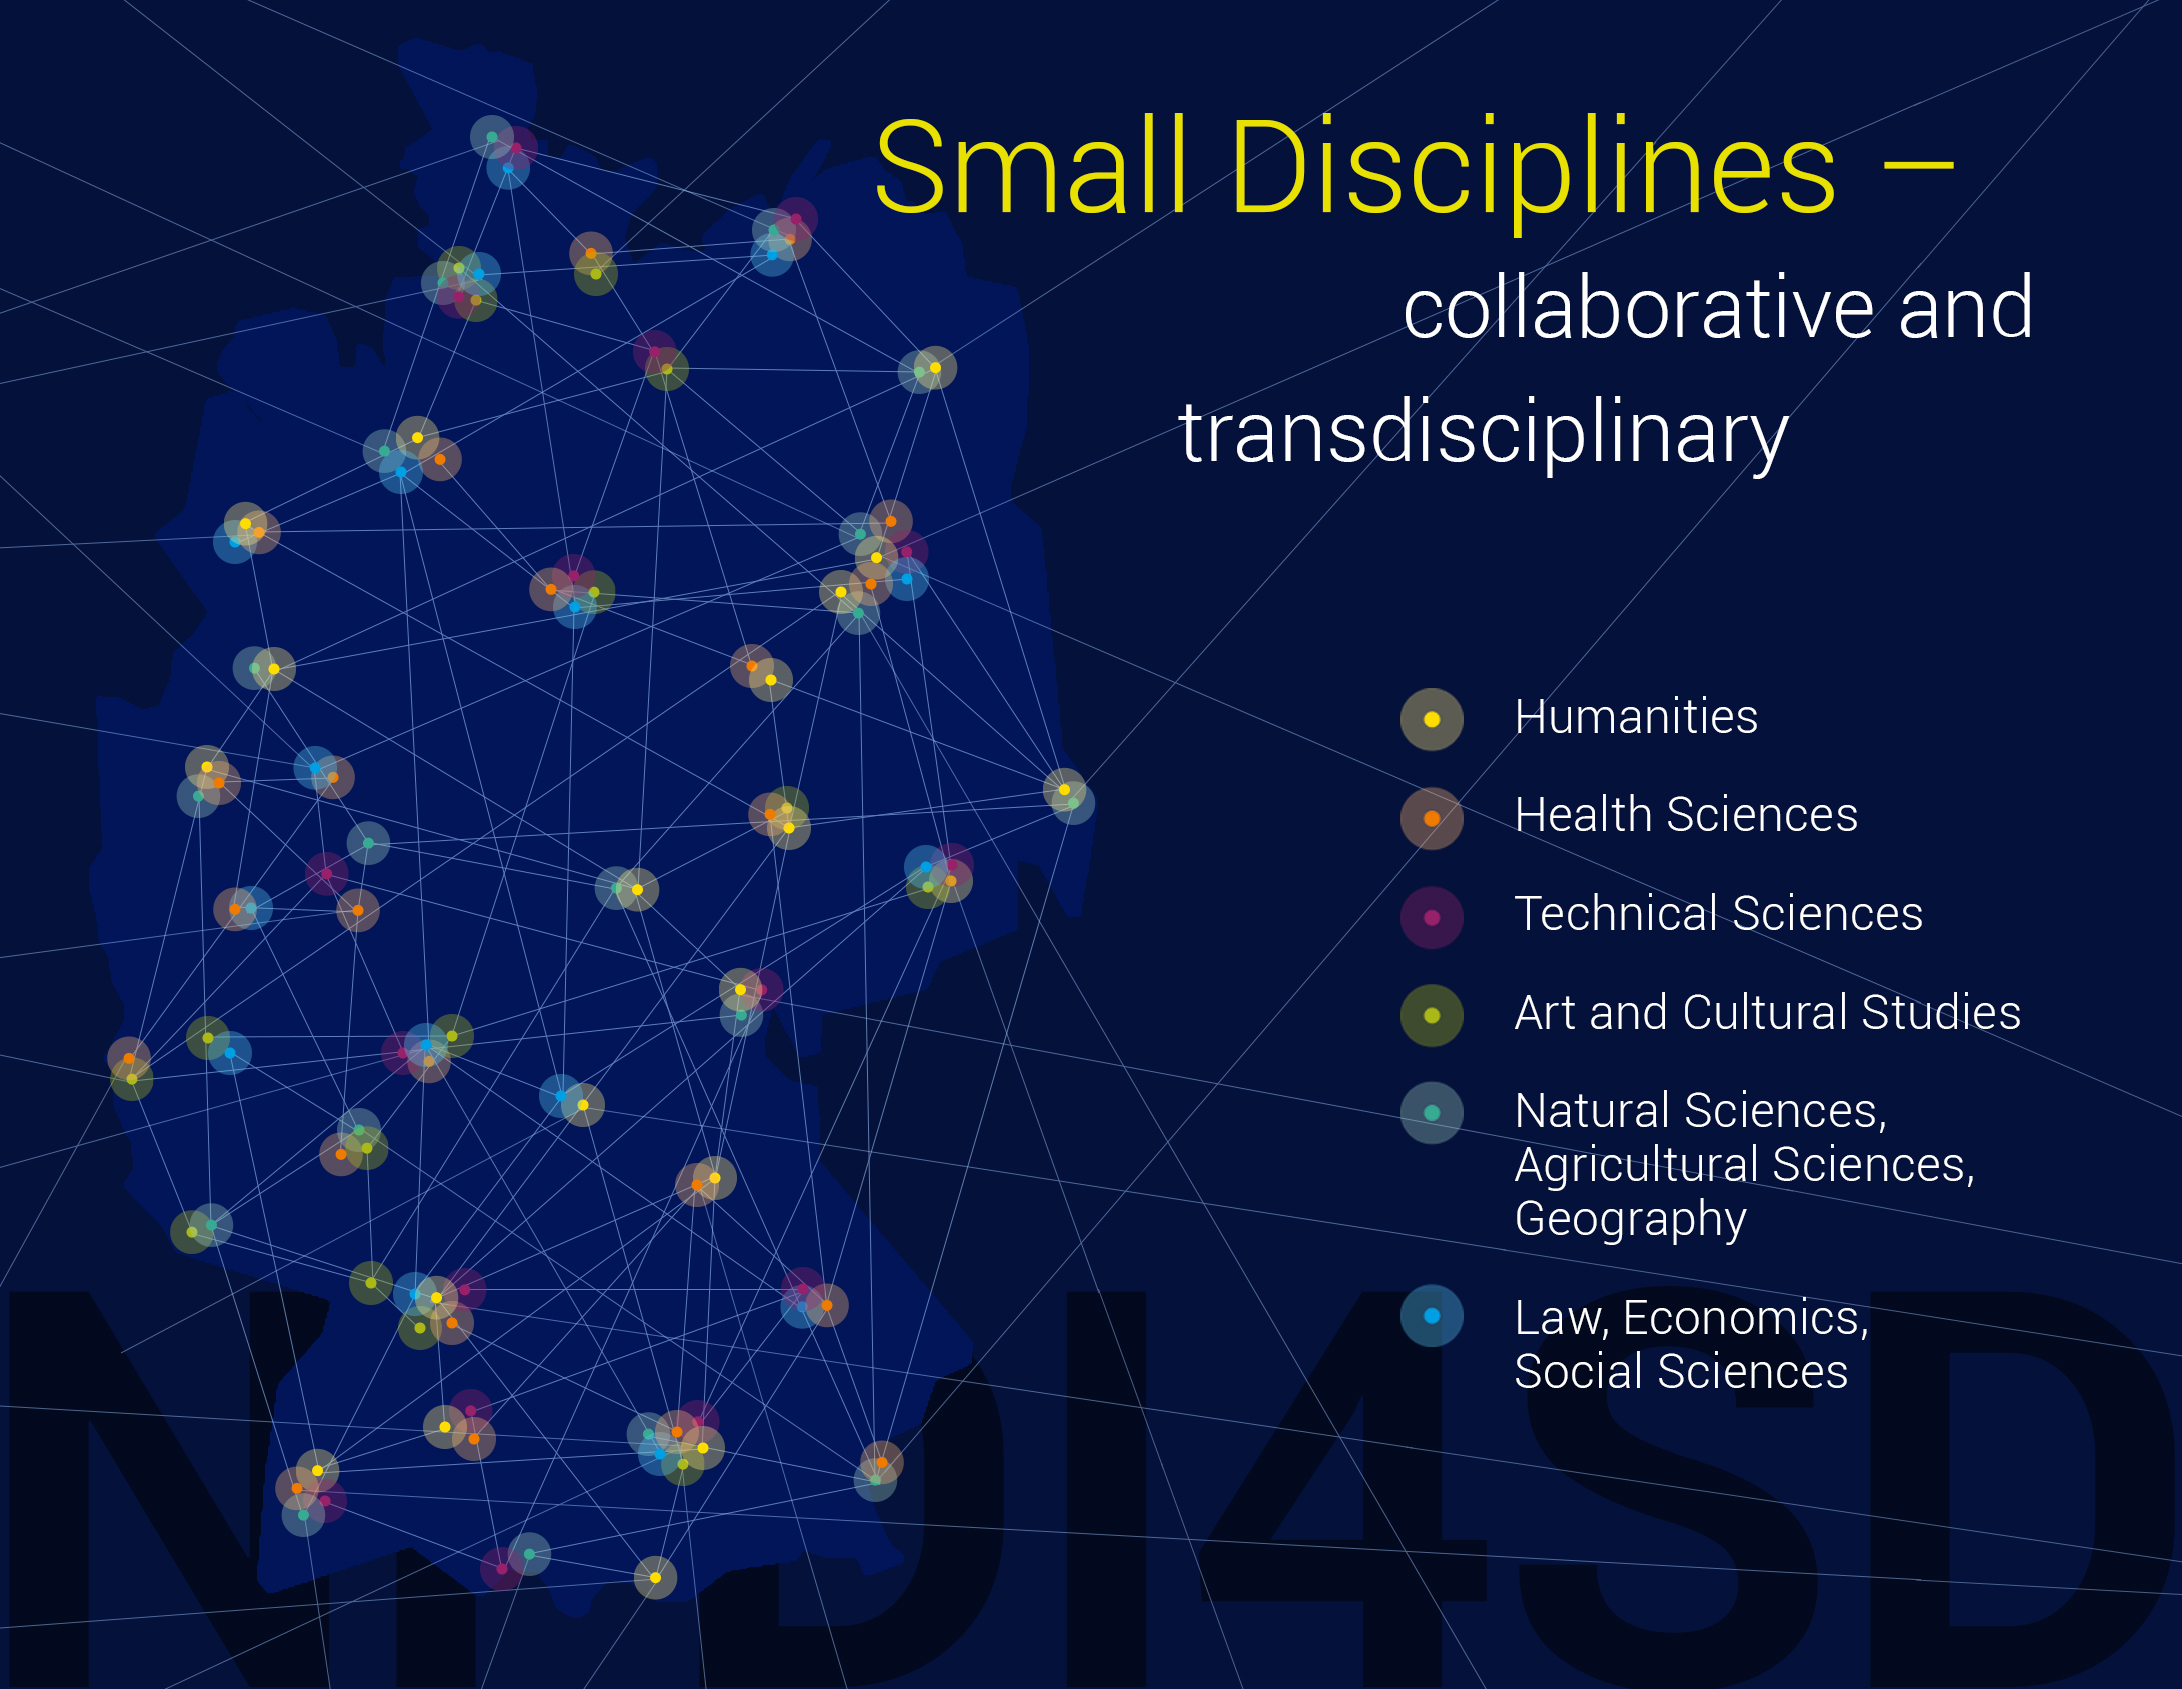
\includegraphics{/Volumes/GGbackup/Dropbox/2020NFDI4SD/Cube/site/concept/assets/NFDI4SD_small-disciplines.jpg}
\caption{sd}
\end{figure}

Ongoing digitalisation and the Open Access movement are transforming the
research process and are greatly increasing the dissemination of
research data. As a result, academic institutions -- such as
universities, research institutes but also smaller groups and agents --
are increasingly committing themselves to managing research data
sustainably and ensuring the interdisciplinary exchange of data. The
initiative to establish a National Research Data Infrastructure, with
the aim of reviewing the systematic planning, collection, processing,
analysis, archiving, publication and exchange of data of various types
to be reused by the scientific community and the general public,
reflects this tremendous structural change.

The Humanities, Cultural Studies and Social Sciences in particular have
been and continue to be faced with new challenges in this regard, since
research data management and standardized data exchange are often less
naturally integrated into their disciplinary divisions and
infrastructures than in the case of the Life Sciences or Natural
Sciences.

In Germany, the so-called small disciplines, which currently include
more than 150 fields of study, mostly in the Humanities, Social and
Cultural Sciences, find the challenges associated with these tasks
particularly difficult to master. Neither the institutions nor the small
disciplines are regarded as being mere sub-disciplines of a larger
discipline.

The long-term funding and continued existence of these disciplines is a
major objective of German higher education and research infrastructure
in general. As the Federal Minister of Education and Research Anja
Karliczek has emphasised: `The small disciplines provide valuable
answers to the many important questions facing our society, not least of
all what holds it together. They create significant knowledge and play a
part in preserving our cultural heritage.'

However , when it comes to setting up modern research data
infrastructures, the small disciplines do not have access to the
resources of the institutions to which, as a rule, they are
organisationally linked, or they cannot gain access to them to the
extent necessary. They also lack the necessary resources and structures
of their own to support the specific needs of their academic community
with regard to modern research data management, to adapting existing
practices to new standards and thus to implementing compatible,
user-oriented concepts for the exchange, backup and reuse of data.

As the Arbeitsstelle Kleiner Fächer or Small Disciplines' Unit of the
Johannes Gutenberg University (JGU) in Mainz has stated, although the
majority of small disciplines belong to the Humanities and Cultural
Studies, which as a whole receive less external funding than other
sectors, they receive a comparatively above-average proportion of
third-party funding (unlike major subjects in Cultural Studies and the
Humanities). This is the case in terms of both the number of
applications and the approved funds, which can be taken to indicate that
the small disciplines do indeed have a high need for additional funding.

At present, there is no standardised higher education policy framework
for the promotion of small disciplines in Germany: some states have
initiated special programmes, while others have no measures at all. The
respective professional associations or foundations have provided
additional funding to the small disciplines.

A further factor to be considered is the highly collaborative and
transdisciplinary working practices of the small disciplines. These are
being investigated in `The Dynamics of Small Disciplines', a research
project funded by the Federal Ministry of Education and Research that
runs from November 2019 to October 2022.

These working methods concern not only the collaborative work undertaken
between several small and/or medium disciplines, but also the teaching
and supervision of young researchers. Given the breadth of topics and
the variety of methods, many of the research questions and topics
covered in the small disciplines can often only be adequately addressed
by interdisciplinary collaboration: innovations are typically achieved
through cross-disciplinary and cross-cultural work in transnational
exchanges. The provision of digital networking, the exchange of research
data and a powerful and user-friendly infrastructure to help realise and
expand these goals in the future are thus of huge importance.

\textbf{The small disciplines: formal criteria}

In order to differentiate the small disciplines from larger departments
and sub-disciplines, the Small Disciplines' Unit at JGU Mainz has
developed a number of criteria

that will be used as the basis for determining the characteristics, user
profiles and specific requirements when using research data. At present,
the unit encompasses 157 small disciplines and 2,311 professorships at
89 locations throughout Germany. These small disciplines fall into six
disciplinary divisions : (1) the Humanities; (2) Health Sciences; (3)
Engineering and Technology; (4) Art and Art History/Aesthetics ; (5)
Natural Sciences, Agricultural Sciences and Geography; and (6) Law,
Economics and Social Sciences. They can be further divided into 19
sections .

More than half of the small disciplines are fields of study in the
Humanities, followed at some distance by the disciplines listed in (5)
and (6).

A decisive factor in this context is that the specific interests of many
of the disciplines grouped together in the six disciplinary divisions
have so far not been addressed separately, if at all, which is due, in
part at least , to a relatively pronounced dynamic in the field: new
small disciplines, such as Digital Humanities or Biodiversity, are
becoming established, while others are losing their status as `small'
disciplines, either because the fields of study are growing or because
they are being absorbed into larger disciplines.

For a field of study to be considered a small discipline:

\begin{itemize}
\item
  there should be no more than three tenured professorships per
  location, although up to two exceptions are possible nationwide. The
  respective discipline will have its own professorships at specific
  appointment grades.
\item
  there should be separate study programmes with a degree at the end.
  The respective academic discipline is represented at German
  universities with its own study programmes (Bachelor's degree,
  Master's degree, diploma, state exam).
\item
  young academics, that is, those who have the potential to obtain a
  doctorate, should be selected and trained. Junior professorships, with
  the prospect of permanent or tenure-track positions, should be
  established.
\end{itemize}

\textbf{Social and communications criteria}

The small disciplines are no longer simply project-oriented but
generally have an international and collaborative focus so that the
thematically and structurally determined research requirements can be
met. They also have a well-defined communications strategy that includes
the use of appropriate types of media as well as a distinct approach for
disseminating information to the general public. This includes:

\begin{itemize}
\item
  the belief in the small discipline as a subject in its own right: the
  professors who represent the respective branch of academic study at
  German universities see their fields of study as an independent
  subject.
\item
  representation by a learned society: the respective branch of
  knowledge is represented by a national or international learned
  society. In exceptional cases, it may be acceptable that the field of
  study is recognized as an independent subject by a learned society.
  Crucially, this is a requirement of various institutions for access to
  funding and on which small disciplines are particularly dependent.
\item
  professional journals and other forms of written communication: there
  should be a national or international specialist publication that
  represents the respective academic discipline.
\end{itemize}

\textbf{Target groups and their requirements}

The main objective of the NFDI4SD is to provide services and an
infrastructure for all the small disciplines and the academic divisions
and groups represented by them so that their scholars can realise their
individual goals and projects through viable research data management. A
service structure set up modularly according to the respective needs and
requirements should be of great help. The various professional,
communications and publication cultures of scholars and scientists need
to be taken into account and should not be restricted by static and
inflexible conditions and processes. In 2019, the sociologist Rudolf
Stichweh described academic disciplines in the context of
differentiation and dedifferentiation movements as highly dynamic
communications systems: digitisation is thus intensifying the increasing
emphasis in present-day research on project planning and a
problem-centred way of working as is today's growing demand for
higher-level professional qualifications.

The NFDI4SD consortium will therefore include researchers from a number
of different disciplines as well as interested institutions in the
development process of the new infrastructure through, among other
things, social media, the development, dissemination and evaluation of
questionnaires on the desired service package and the tendering and
funding of pilot projects. The knowledge and experience gained will be
incorporated into the structure and development process of the NFDI4SD
and will be evaluated successively. The aim is to make research data
reusable through a number of different action strategies in order to
avoid the data being lost owing to a lack of time, expertise or
financial means.

At this juncture, another feature of the NFDI4SD makes itself known:
projects at different stages of development, of varying sizes and with
varying funding periods are explicitly addressed, from qualification
projects, such as university theses and dissertations, to larger
research groups at institutions or universities.

The publication of research findings, particularly in the case of
doctoral theses, has, in many disciplines, so far been the primary
indicator of the success of a research project, while the underlying
data were not contextualized or systematically indexed. This meant that
the data could not be cited in other academic studies without first
having been reworked. In more extensive interdisciplinary research
projects and collaborative work, the insights and partial findings
gained through communicating with others and making evaluations from a
number of different perspectives are of particular importance as they
facilitate the publication of research data and partial findings. As a
consequence, a stronger dynamic is developed, which benefits the entire
research process.

\textbf{Desiderata}

\textbf{D1} Review the sequential planning approach, which tends to
place publication at the end of a research process and thus usually
beyond the funding period

\textbf{D2} Create an infrastructure for archiving and publishing the
data in the long term

\textbf{D3} Integrate the research data into a network of global data
resources that supplement each other

\textbf{D4} Register applicable software solutions for standard
computational workflows

\textbf{D5} Integrate expertise outside academia into a data network of
specialized resources

\textbf{D6} Disseminate the research findings to the general public.
Develop and implement quick and stable deployment strategies

\textbf{Additional references }

\begin{enumerate}
\def\labelenumi{\arabic{enumi}.}
\tightlist
\item
  \href{https://www.kleinefaecher.de/beitraege/blogbeitrag/dokumentation-zur-tagung-kleine-faecher-entwicklungen-strategien-perspektiven.html}{Arbeitsstelle
  Kleine Fächer: Tagung „Kleine Fächer: Entwicklungen -- Strategien --
  Perspektiven``, 12./13.09.2019},
\item
  \href{https://www.kleinefaecher.de/fileadmin/user_upload/img/Abschlusstagung_2019_Der_Blick_der_Universitaetsgeschichte_auf_die_Kleinen_Faecher_Paletschek.pdf}{Sylvia
  Paletschek: Der Blick der Universitätsgeschichte auf die Kleinen
  Fächer, Tagung „Kleine Fächer: Entwicklungen -- Strategien --
  Perspektiven``, 2019}
\item
  \href{https://www.kleinefaecher.de/fileadmin/user_upload/img/Abschlusstagung_2019_Strategische_Weiterentwicklung_Kleiner_Faecher_Dreyer.pdf}{Mechthild
  Dreyer: Strategische Weiterentwicklung Kleiner Fächer. Resümee der
  Empfehlungen der Workshops Januar/Oktober 2018}
\item
  \href{https://www.kleinefaecher.de/fileadmin/user_upload/img/Kartierungsbericht_2019.pdf}{Arbeitsstelle
  Kleine Fächer: Kartierungsbericht 2019}
\item
  \href{https://www.volkswagenstiftung.de/sites/default/files/downloads/2019-05\%20Bericht_Fächer-in-Bewegung.pdf}{Vera
  Szöllösi-Brenig: Bericht zum Symposium ``Fächer in Bewegung --
  Differenzierung und Entdifferenzierung im System der Wissenschaft?'',
  2019}
\item
  \href{https://www.kleinefaecher.de/fileadmin/user_upload/img/Abschlusstagung_2019_Eroeffnungsvortrag_Kleine_Faecher_grosse_Aussichten_Loprieno.pdf}{Antonio
  Loprieno: Kleine Fächer und große Aussichten. Fachtagung der
  Arbeitsstelle Kleine Fächer, Mainz 2019}
\item
  \href{https://www.bmbf.de/foerderungen/bekanntmachung-2604.html}{Förderrichtlinen
  für Kleine Fächer, BMBF, 25.07.2019}
\item
  \href{https://www.dropbox.com/s/6yza1yuih8cvjzx/Programm_Digitalisierungsworkshop_kleine_F\%C3\%A4cher_Nov_digital.pdf?dl=0}{Informations-
  und Vernetzungsworkshop, Digitalisierung in Lehre und Forschung
  kleiner Fächer im Rahmen des Projekts „Die Dynamik kleiner Fächer`` 5.
  November 2020}
\end{enumerate}

\hypertarget{research-data-1}{%
\section{Research Data}\label{research-data-1}}

\begin{figure}
\centering
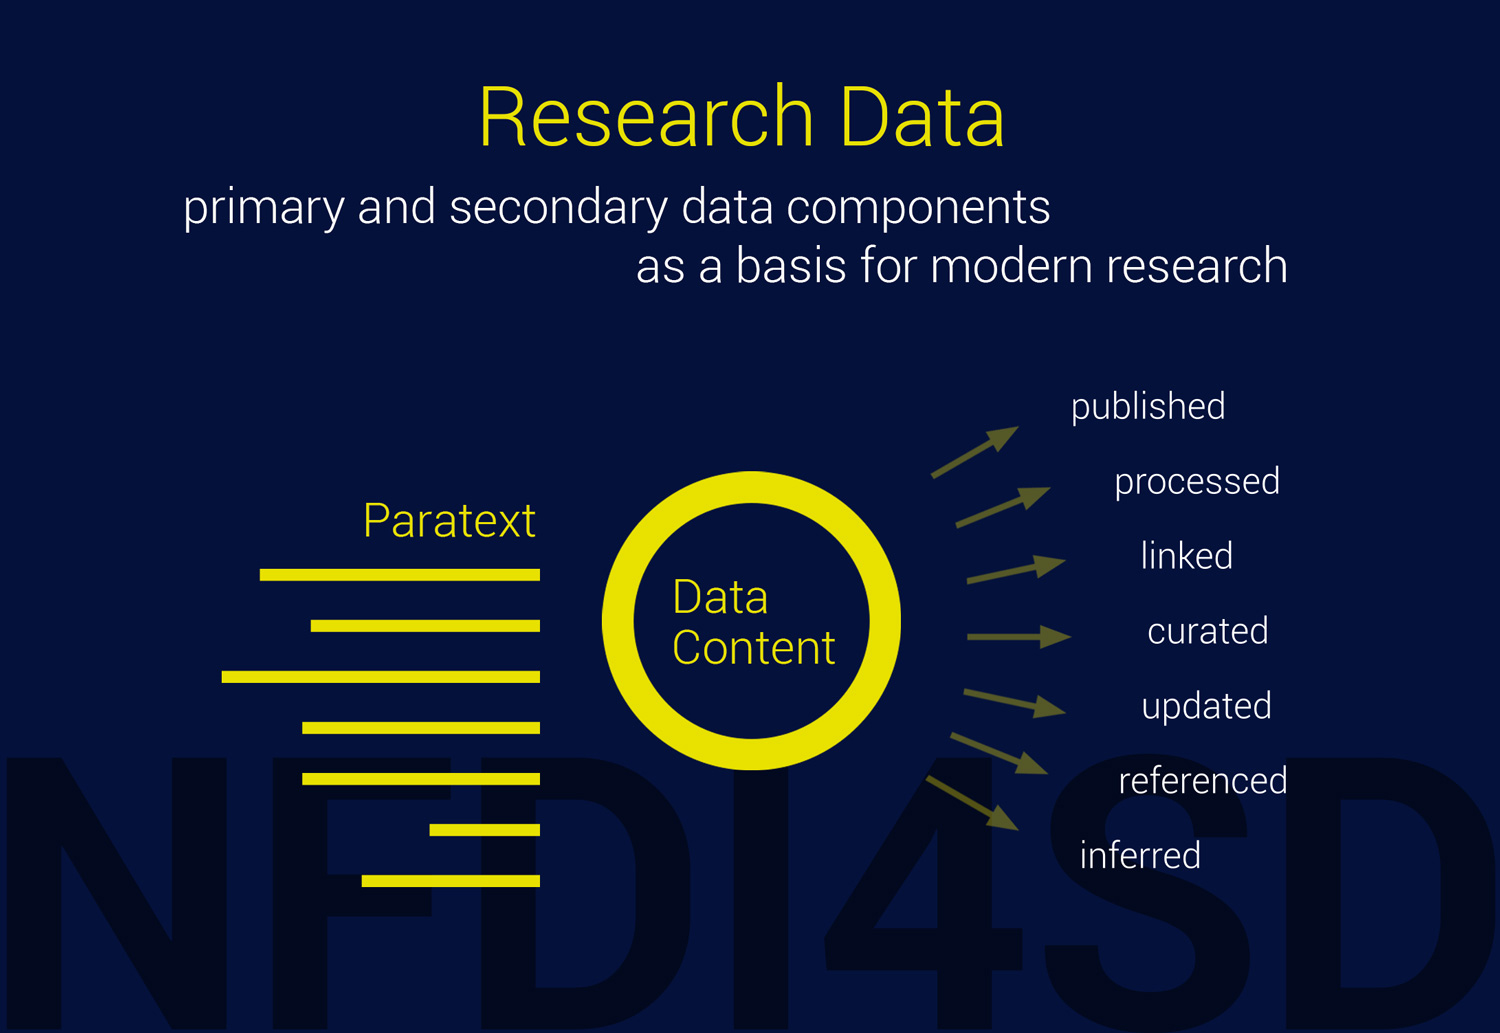
\includegraphics{/Volumes/GGbackup/Dropbox/2020NFDI4SD/Cube/site/concept/assets/NFDI4SD_research-data.jpg}
\caption{sd}
\end{figure}

\hypertarget{epistemology-of-research-data}{%
\subsection{Epistemology of research
data}\label{epistemology-of-research-data}}

Research data are not an invention of the digital age: since antiquity
they have been published and used in the history of scholarship as a
distinct type of information. The localities and paths of the ancient
world were listed in data catalogues, such as Ptolemy's
\emph{Geography}, and scholars determined the constellation of the stars
with the help of Ptolemy's \emph{Handy Tables}. Early calendars and the
dating of religious festivals were also based on research data, while
encyclopaedias provided summaries of standardised knowledge. Extensive
collections of research data created the success of modern scholarship
and science in combination with the development of grand theories,
although, as these collections were mostly collaborative projects, they
often did not bear an author's name. Research data are epistemically
verified with the greatest of care in all academic cultures. They are
bodies of knowledge that are regularly examined to identify errors as
quickly as possible and to mark the validated data. Thus, research data
are not simply information that is disseminated on the Internet in our
digital age, linked to other data and made accessible irrespective of
its truthfulness. Nor are they `closed data', which, like rarefied
treasures, are only accessible to the privileged few.

The concept of knowledge was introduced by scholars to classify this
special status of information about society and the world. With the
generic nature of theory, we can characterize research data as the
description of any class of objects that qualifies as knowledge.
Research data as knowledge about the properties of research objects
which have been methodologically evaluated by the academic community can
therefore be distinguished from arbitrary information: research data are
collaboratively, openly and critically examined; they represent a claim
of validity that can be revised at any time. The organisation of
scholarly communication and the ethos of dealing with knowledge are
optimised in order to minimise errors. These established methodological
mechanisms should apply to the research data of all disciplines.

This special status of research data, together with all the academic
disciplines, including in particular the so-called small disciplines, is
the main focus of the NFDI4SD's challenge of developing an appropriate
research data infrastructure.

\begin{awesomeblock}[magenta]{1pt}{RD1}{magenta} Scholars and scientists consider research data to be fallible knowledge: they can be justified and can then serve as the basis for justifying statements; they can also qualify as epistemic states. To this end, they must be computationally identifiable at all times, independently of their symbolic form. All epistemic qualifications need to be transparent.\end{awesomeblock}

All the additional attributes that are used to handle research data as
knowledge can be synthesised. Research data can be differentiated
according to the components of the data's content, the metadata and the
epistemic knowledge claims qualification. The content of research data
refers to the characteristics of the research objects described by the
data. Research data always include both content and its additional
attributes. As a result, an infrastructure of research data must assure
and maintain data integrity.

We can draw an analogy between our understanding of research data and
the concept of paratext ((``Annika Rockenberger, PhiN 76/2016: 20.''
\protect\hyperlink{ref-zotero-40395}{n.d.})), which has been debated in
the past few years: according to the philologically based concept
introduced by Gérard Genette (1930--2018), paratexts are those elements
that have been added to the main text of an (originally literary) work
and which decisively influence and control the reception and
distribution of the work. These elements include information on the
author, the publisher, the title, preface, acknowledgements,
advertising, and so forth. (Genette
\protect\hyperlink{ref-genette1997}{1997}) The concept of paratext,
which directs greater attention to production processes and to cases of
authorisation, was later extended to include various types of text and
new media formats. In the context of the digitisation of research data,
this means that the verification, authorisation and permanent
accessibility of research data will have a particularly decisive
influence on the adherence and further development of national and
international standards and quality requirements.

\begin{awesomeblock}[magenta]{1pt}{RD2}{magenta} Research data are composed of content, metadata and epistemic attributes. All the information on the data sources, such as main texts and paratexts, is unified within the research data. The composition of the data needs to adhere to epistemic principles in order to enhance the way in which knowledge is obtained, accessed and maintained.\end{awesomeblock}

It was the physicist and philosopher Hans Reichenbach (1891--1953) who
codified the distinction between the context of discovery and the
context of justification in connection with critically evaluating
statements. The context of discovery takes into account the causes that
lead to new insights being formed and the evaluation of scientific
evidence. The basis for the justification of statements must be
differentiated from the discovery of statements, regardless of whether
they are theoretical hypotheses or the content of research data.
Researchers who are looking for new answers and who create and use
research data for this purpose, focus on the context of discovery.
However, in doing so they overlook the fact that a discovery process is
always based on knowledge that has already been justified. Research data
are validated particularly carefully if they are being prepared for
publication during the research process.

\begin{awesomeblock}[magenta]{1pt}{RD3}{magenta} The value of research data must always be assessed according to how it will be reused by others and not from the perspective of the first person involved in the discovery process.\end{awesomeblock}

The justification of knowledge -- and thus the validity of research data
-- is a collaborative task of the entire research community. Therefore,
the research data infrastructure must provide the means to track the
provenance of research data as well as the epistemic dependence on
tertiary sources. This is rarely guaranteed at present.

\begin{awesomeblock}[magenta]{1pt}{RD4}{magenta} The justification of the data by other research data should be as transparent and comprehensible as possible. A ‘dependency graph’ can show how research data is connected to other research data and thus clarify the epistemic dependencies between them. The academic assumptions that determine the validity of the research data should be clearly identifiable.\end{awesomeblock}

It thus follows that newly acquired data within an innovative research
organisation must be made available to other academics as quickly and
completely as possible if the data is to be epistemically possible. This
act of transferring research data from the hands of individual
researchers who are working in the context of discovery to the public
has its own special term: \emph{academic publication}.

\begin{awesomeblock}[magenta]{1pt}{RD5}{magenta} Publication. The publishing of research data is the act of handing over compiled findings of data that were made in the discovery context to the academic community. Only then do the findings become justified knowledge. Research data is given the status of empirical findings only once they have been published. Research data publication leads to citable data sets, which are listed in the bibliographies of other authors, such as in current research literature.\end{awesomeblock}

The consequence is that research data publication is now being
considered as early as possible in management planning. A strict
sequence of processes, in which the publication of research data is
planned only after the completion of a project and after all other
activities have been finalised, is thus no longer logical from the point
of view of academic theory; indeed, it adversely affects innovative
research. The modified workflow of data publication and data citation
will result in research projects gaining greater visibility, while the
publication of one's own data will significantly increase the impact of
the project and the people involved in it.

\begin{awesomeblock}[magenta]{1pt}{RD6}{magenta} Citing research data. The origin of reused research data should always be cited. Research data should be cited, like any other scholarly source, in bibliographies or lists of references. The format of a data citation also resembles the reference styles of other bibliographical sources. Citations can be managed and administered in citation databases or by using citation tools.\end{awesomeblock}

During the course of a research project, a great deal of research data
is created in relation to other data. The new data are annotated, linked
or are used in other ways to further research. The scope of these
research data is huge, yet currently very little of these data are
published. These data sets considerably increase the usefulness of the
linked data.

\begin{awesomeblock}[magenta]{1pt}{RD7}{magenta} Enhancing research data. Modern research projects create a rich and additional amount of research data during the research process.\end{awesomeblock}

\hypertarget{institutional-consequences-the-use-of-fair-principles}{%
\subsection{Institutional consequences: the use of FAIR
principles}\label{institutional-consequences-the-use-of-fair-principles}}

We understand the FAIR data principles to be a framework for developing
an infrastructure that serves research data as a knowledge base with the
purpose of creating a collaborative and open science.

In order to create the conditions for such a framework, a number of
leading international research associations and institutions committed
themselves to implementing the FAIR data principles. Increasingly, many
funding bodies only allocate funds to projects that fulfil FAIR
conditions. Today, however, these conditions cannot be guaranteed by
researchers alone: research projects in the small disciplines that are
managed in an agile and collaborative way in particular do not tend to
have the resources to meet the special requirements of providing and
using research data. A research-based infrastructure will be needed.

The FAIR principles can be interpreted in a variety of ways, but we
intend to follow the proposals of the GO FAIR initiative,\footnote{\href{https://www.go-fair.org/go-fair-initiative/}{go
  fair}}the vision of which is to foster `the coherent development of
the global Internet of FAIR Data \& Services (IFDS), with the main focus
on early developments in the European Open Science Cloud
(EOSC).'\footnote{\href{https://www.go-fair.org/fair-principles/}{Go
  fair principles}}

\begin{awesomeblock}[magenta]{1pt}{RD8}{magenta} The FAIR principles (reproduced below from the GO FAIR website) regulate the technical implementation of research data. The NFDI4D will use these guidelines to implement its research data infrastructure. The guidelines are intended to ‘improve the Findability, Accessibility, Interoperability and Reuse of digital assets’:\end{awesomeblock}

\hypertarget{findable}{%
\subsection{Findable}\label{findable}}

\begin{quote}
The first step in (re)using data is to find them. Metadata and data
should be easy to find for both humans and computers. Machine-readable
metadata are essential for automatic discovery of datasets and services,
so this is an essential component of the FAIRification process.
\end{quote}

\begin{quote}
F1. (Meta)data are assigned a globally unique and persistent identifier
\end{quote}

\begin{quote}
F2. Data are described with rich metadata (defined by R1 below)
\end{quote}

\begin{quote}
F3. Metadata clearly and explicitly include the identifier of the data
they describe
\end{quote}

\begin{quote}
F4. (Meta)data are registered or indexed in a searchable resource
\end{quote}

\hypertarget{accessible}{%
\subsection{Accessible}\label{accessible}}

\begin{quote}
Once the user finds the required data, s/he needs to know how can they
be accessed, possibly including authentication and authorisation.
\end{quote}

\begin{quote}
A1. (Meta)data are retrievable by their identifier using a standardised
communications protocol
\end{quote}

\begin{quote}
A1.1 The protocol is open, free, and universally implementable
\end{quote}

\begin{quote}
A1.2 The protocol allows for an authentication and authorisation
procedure, where necessary
\end{quote}

\begin{quote}
A2. Metadata are accessible, even when the data are no longer available
\end{quote}

\hypertarget{interoperable}{%
\subsection{Interoperable}\label{interoperable}}

\begin{quote}
The data usually need to be integrated with other data. In addition, the
data need to interoperate with applications or workflows for analysis,
storage and processing.
\end{quote}

\begin{quote}
I1. (Meta)data use a formal, accessible, shared, and broadly applicable
language for knowledge representation
\end{quote}

\begin{quote}
I2. (Meta)data use vocabularies that follow FAIR principles
\end{quote}

\begin{quote}
I3. (Meta)data include qualified references to other (meta)data
\end{quote}

\hypertarget{reusable}{%
\subsection{Reusable}\label{reusable}}

\begin{quote}
The ultimate goal of FAIR is to optimise the reuse of data. To achieve
this, metadata and data should be well-described so that they can be
replicated and/or combined in different settings.
\end{quote}

\begin{quote}
R1. (Meta)data are richly described with a plurality of accurate and
relevant attributes
\end{quote}

\begin{quote}
R1.1. (Meta)data are released with a clear and accessible data usage
license
\end{quote}

\begin{quote}
R1.2. (Meta)data are associated with detailed provenance
\end{quote}

\begin{quote}
R1.3. (Meta)data meet domain-relevant community standards
\end{quote}

Many of the principles mentioned above are open to a number of
interpretations. As a result, no technical specifications can be deduced
from these regulations. Expressions for the release of and access to
data, such as `released' and `accessible', do not give enough
information on the procedures. The NFDI4SD's partner Zenodo, which is
hosted by CERN, has developed its own `best effort principles'. (s) A
substantial part of the publishing of small- and medium-sized research
data collections is expected to be done on the Zenodo platform. Larger
collections will be stored in separate data repositories. To begin with,
the larger collections will carry out Zenodo's implementation proposals.

\hypertarget{paratext}{%
\section{Paratext}\label{paratext}}

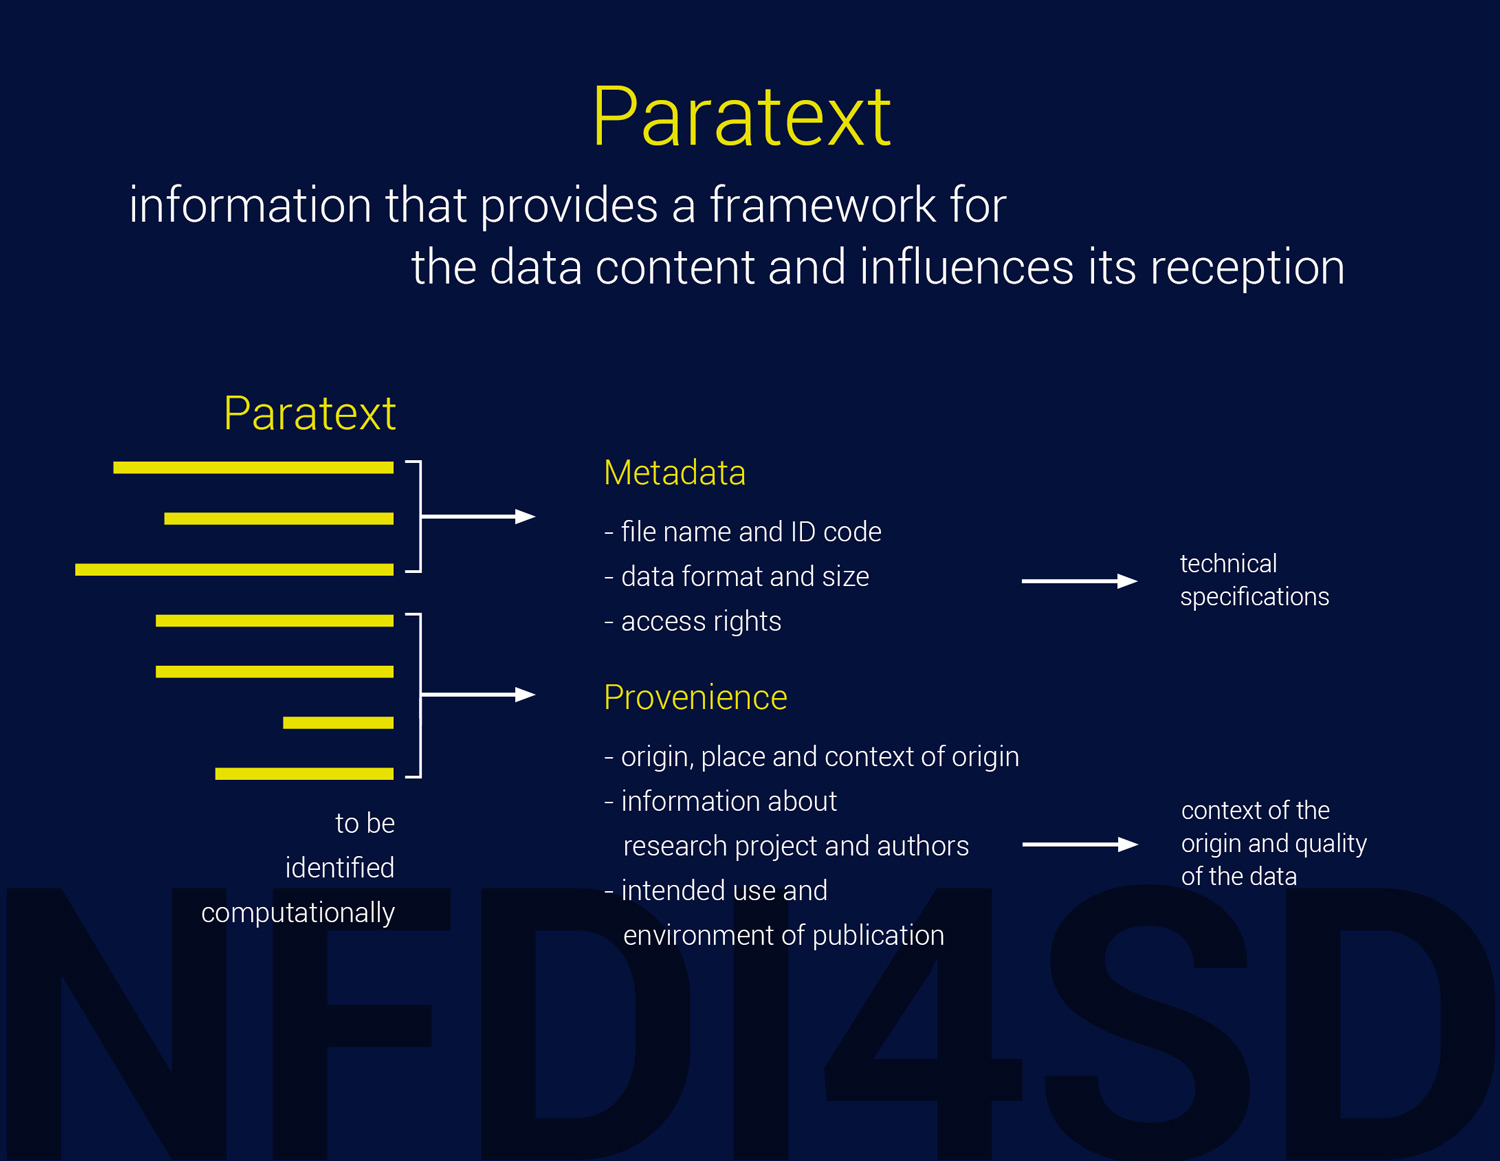
\includegraphics{/Volumes/GGbackup/Dropbox/2020NFDI4SD/Cube/site/concept/assets/NFDI4SD_paratext.jpg}

\hypertarget{metadata}{%
\subsection{Metadata}\label{metadata}}

Besides the content data, the paratext of research data contains
different types of additional metadata. Citing the recommended metadata
of the RDA,\footnote{\href{http://rd-alliance.github.io/metadata-directory/}{rda
  Metadata Standards Directory Working Group}} and OpenAIRE:\footnote{\href{https://www.openaire.eu/what-is-metadata\#:~:text=Some\%20specific\%20examples\%20of\%20metadata,economic\%20sciences\%2C\%20including\%20survey\%20data}{metadataOpenAIRE}}

\begin{quote}
Metadata is data providing information about data that makes findable,
trackable and (re)usable. It can include information such as contact
information, geographic locations, details about units of measure,
abbreviations or codes used in the dataset, instrument and protocol
information, survey tool details, provenance and version information and
much more.
\end{quote}

The recommended set of paratext data will be discussed at the beginning
of the NFDI4SD in workshops and expert consultations. Metadata will
satisfy the required core (e.g.~Dublin core, Datacite and OpenAIRE). We,
therefore, apply the proposal of
\href{http://schema.datacite.org/meta/kernel-4.3/doc/DataCite-MetadataKernel_v4.3.pdf}{Datacite}.
We share the experience that in the important data aggregation such as
the definition of metadata, standardised ontologies only play a
subordinate role so far. A standardisation of terminology and meaning
will still be a tightly controlled part of the data preparation process.

\hypertarget{ontologien-cidoc-referenzdaten}{%
\subsection{Ontologien / CIDOC /
Referenzdaten}\label{ontologien-cidoc-referenzdaten}}

NFDI4D wird ein reichhaltiges Portfolio von machinell verarbeiteten
Ontologien zur Verfügung stellen (vergleichbar mit
\href{https://arches.readthedocs.io/en/latest/ontologies-in-arches/}{Achres}),
z.B. CRM (Conceptual Reference Model
(\href{http://www.cidoc-crm.org/}{CIDOC})). Das von NFDI4D bevorzugte
bottom-up Modell der semantischen Frameworks und ihrer inferentiellen
Verarbeitung sieht immer ein Prüfung ihrer Anwendungsbereiche durch die
Projekt selbst vor. Die darauf aufbauenden machine learning algorithmen
müssen immer ihre Qualitätsmetriken am annotierten
Referenzdatenbeständen ausweisen. Diese Referenzdaten sind selbst im
Idealfall publizierte, manuell von den Forschern ausgewählte und
geprüfte Forschungsdaten.

Following considerations might be taken into account:

\begin{itemize}
\tightlist
\item
  Paratext data will best be coded as
  \href{https://json-ld.org/}{JSON-LD} format, which as a lightweight
  Linked Data format allows a standardized API for complex hierarchical
  data structures. Its standards are ideal for an interoperable API,
  REST-services and Web interface.\footnote{\href{https://json-ld.org/learn.html}{Information
    about json-ld linked data}}Transformations into other formats and
  standards are planned.
\item
  Core metadata, as required by ZENODO and generic data repositories,
  will be included in the set of metadata.
\item
  Paratext will consist of the provenance of data to allow the
  composition of a data dependency graph. It will enable functions for
  the NFDI4SD registry to administer data dependencies and informative
  navigation through data repositories to the researcher.
\item
  Many data provider - e.g.~Bayerischer Staatsbibiothek München - as a
  pivotal content provider for digital ressources, has tagged
  exceptionally well their more than 2.5 mio digital objects and
  provides various RDF and XML structured metafiles. Their schema will
  be transparently used for the subsequent processing of research data
  for our researcher. A maximum of coherence of data and metadata is
  intended.
\item
  Meaningful data APIs will be created along the lines of
  \href{https://rollout.io/blog/json-ld-building-meaningful-data-apis/}{API}
  considerations.
\item
  Machine learning tools of the NFDI4SD will supply flexible mapping
  between user-specific terminology and data standards.
\item
  Sufficient documentation of data, their origin, units, explanation of
  terms and cross-linking to standards of definition are recommended and
  will be assisted by appropriate tools using research feedback from the
  specific research community.
\item
  There is a discussion about the advantage of
  \href{https://ddialliance.org/announcement/public-review-structured-data-transformation-language-sdtl}{Structured
  Data Transformation (SDTL)} which addresses the issue of data
  provenance.\footnote{\href{http://c2metadata.gitlab.io/sdtl-docs/master/summary/}{Version
    1.0} and \href{http://c2metadata.org/}{c2meta}} A proposal is under
  review.
\end{itemize}

\# Standards and NFDI4D's \emph{Standards-Companion}

The proven and widely used services such as Zenodo, reference data,
programming languages and ontologies already presuppose a rich set of
standards and norms for the data used.

Some specific examples of metadata standards, both general and domain
specific are:

\begin{itemize}
\tightlist
\item
  Dublin Core - domain agnostic, basic and widely used metadata standard
\item
  DDI (Data Documentation Initiative) - common standard for social,
  behavioral and economic sciences, including survey data
\item
  EML (Ecological Metadata Language) - specific for ecology disciplines
\item
  ISO 19115 and FGDC-CSDGM (Federal Geographic Data Committee's Content
  Standard for Digital Geospatial Metadata) - for describing geospatial
  information
\item
  MINSEQE (MINimal information about high throughput SEQeuencing
  Experiments) - Genomics standard
\item
  FITS (Flexible Image Transport System) - Astronomy digital file
  standard that includes structured, embedded metadata
\item
  MIBBI - Minimum Information for Biological and Biomedical
  Investigations Where no appropriate, formal metadata standard exists,
  for internal use, writing ``readme'' style metadata is an appropriate
  strategy. If you need more information, check the following resources:
\item
  DCC Metadata Standards
\item
  RDA Metadata Directory
\end{itemize}

Other standards and ontologies:

\begin{itemize}
\tightlist
\item
  Zenodo API
\item
  PID systems
\item
  JSON-LD
\item
  UTF 8
\item
  CIDOC\footnote{{[}@{]}}
\item
  Schema.org
\end{itemize}

Researchers are not expected to master all these standards themselves
and to be able to judge the advantages and disadvantages of other
standards.

Disciplines therefore develop or use their own specific terminologies,
whereby research data distributed over various contexts of origin
accumulates a conceptual vagueness that creates difficulties in the
uncritical use of simple terminology. Linked Open Data (LOD) should
therefore go beyond the sole use of ontologies and move from the
possibilities of machine learning to the tested use of vague concepts.
Mees, Thiery and Unold have convincingly pointed out use cases of
provincial Roman archaeology and many others no subject.\footnote{(Unold,
  Thiery, and Mees \protect\hyperlink{ref-unold2019}{2019})}

In order to offer the development as well as the use of the rich
standards to researchers as a service, NFDI4SD is developing a
\emph{Standards-Companion}. Analogous to the Companion on legal
standards, NFDI4SD is developing a Standards-Companion, which classifies
the registered research data with the means of machine learning on the
application of standards and directly generates an automated report on
the standards used, their reference pages and further literature via the
virtual research bench. Alternative standard concepts are also reported.
The Standards-Companion constantly updates its own database and in this
way ensures the harmonisation of research data. The data sources for the
Standard-Companion are in particular

\begin{itemize}
\tightlist
\item
  Formal models of the standards
\item
  Labeled data for machine learning
\end{itemize}

\hypertarget{provenience}{%
\subsection{Provenience}\label{provenience}}

Data Provenience will become part of the paratext of research data. It
will be gathered by compiling a dependency graph between research data
objects as described in either narrative publications or the analysis of
computational notebooks. Each research data object will carry a unique
identifyer and reference in research publication establish the
dependencies between them. NFDI4SD registry will build up a large
dependency graph for research data that will be the basis of supporting
the cataloging and reuse of research data.

\hypertarget{nfdi4sd-services}{%
\chapter{NFDI4SD Services}\label{nfdi4sd-services}}

\hypertarget{portfolio-of-services}{%
\section{Portfolio of services}\label{portfolio-of-services}}

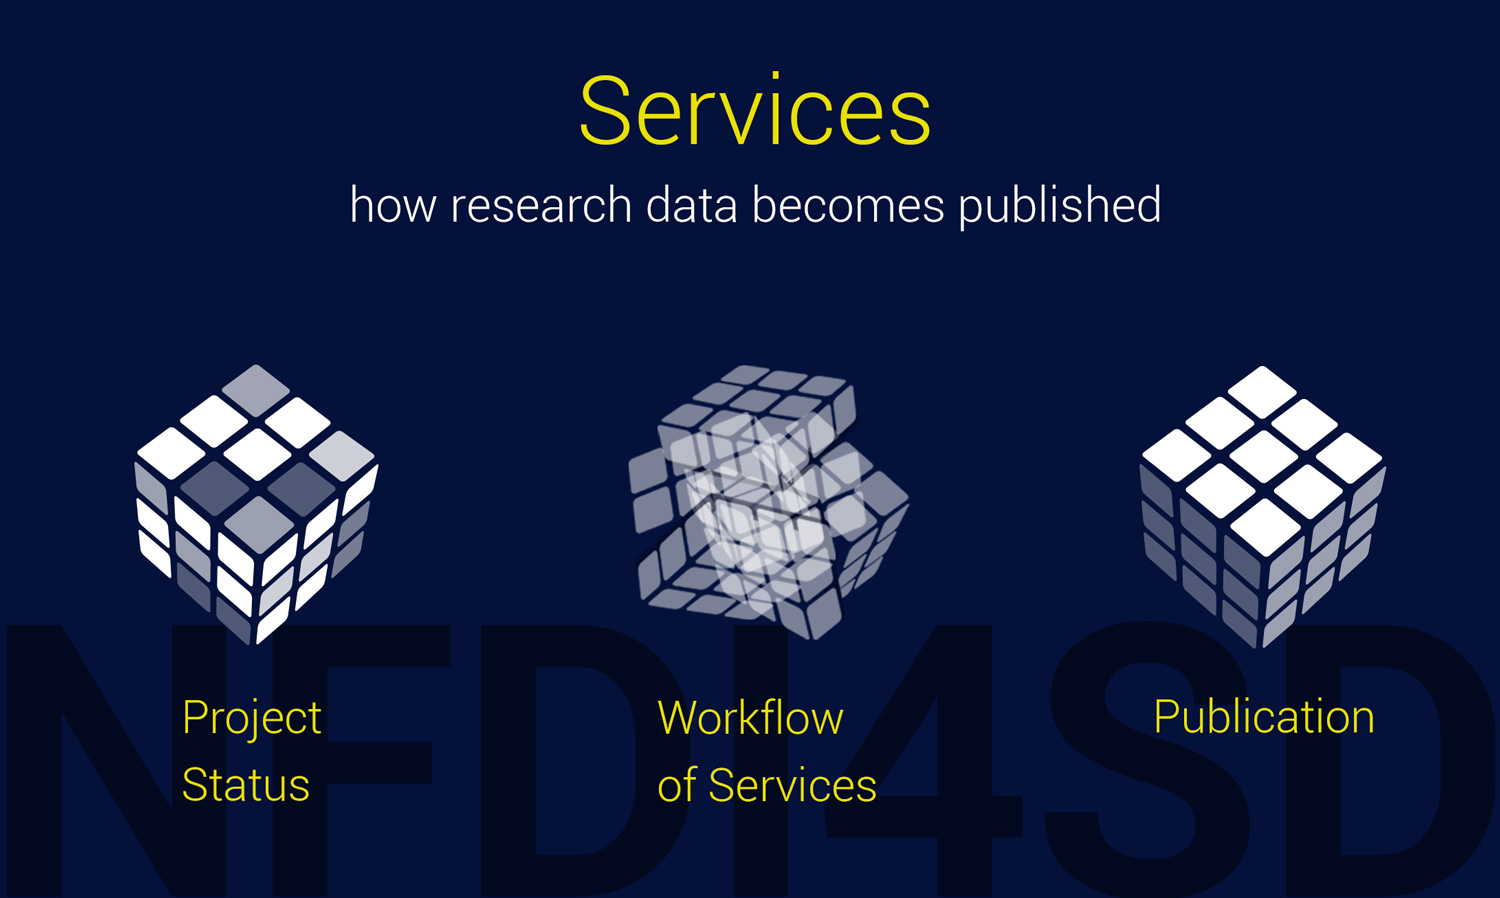
\includegraphics{/Volumes/GGbackup/Dropbox/2020NFDI4SD/Cube/site/services/assets/NFDI4SD_services.jpg}

Services unterstützen die workflow der Bearbeitung von Forschungsdaten.
Die meisten NFDI4D Services werden als Programmpakete in den
Datenprozesse von computational notebooks aufgerufen. Es werden viele
der open als open Sie sind in Service-Klassen unterschieden, die
wiederum eine Reihe von einzelnen Modulen enthalten. Ihre Parameter
erlaubten ein hoch flexibles Pipelining der Services, so dass Ketten von
Services miteinander verschränkt werden können und automatisierte
Bearbeitungspipelines für Forschungsdaten eingerichtet werden können.

\begin{figure}
\centering
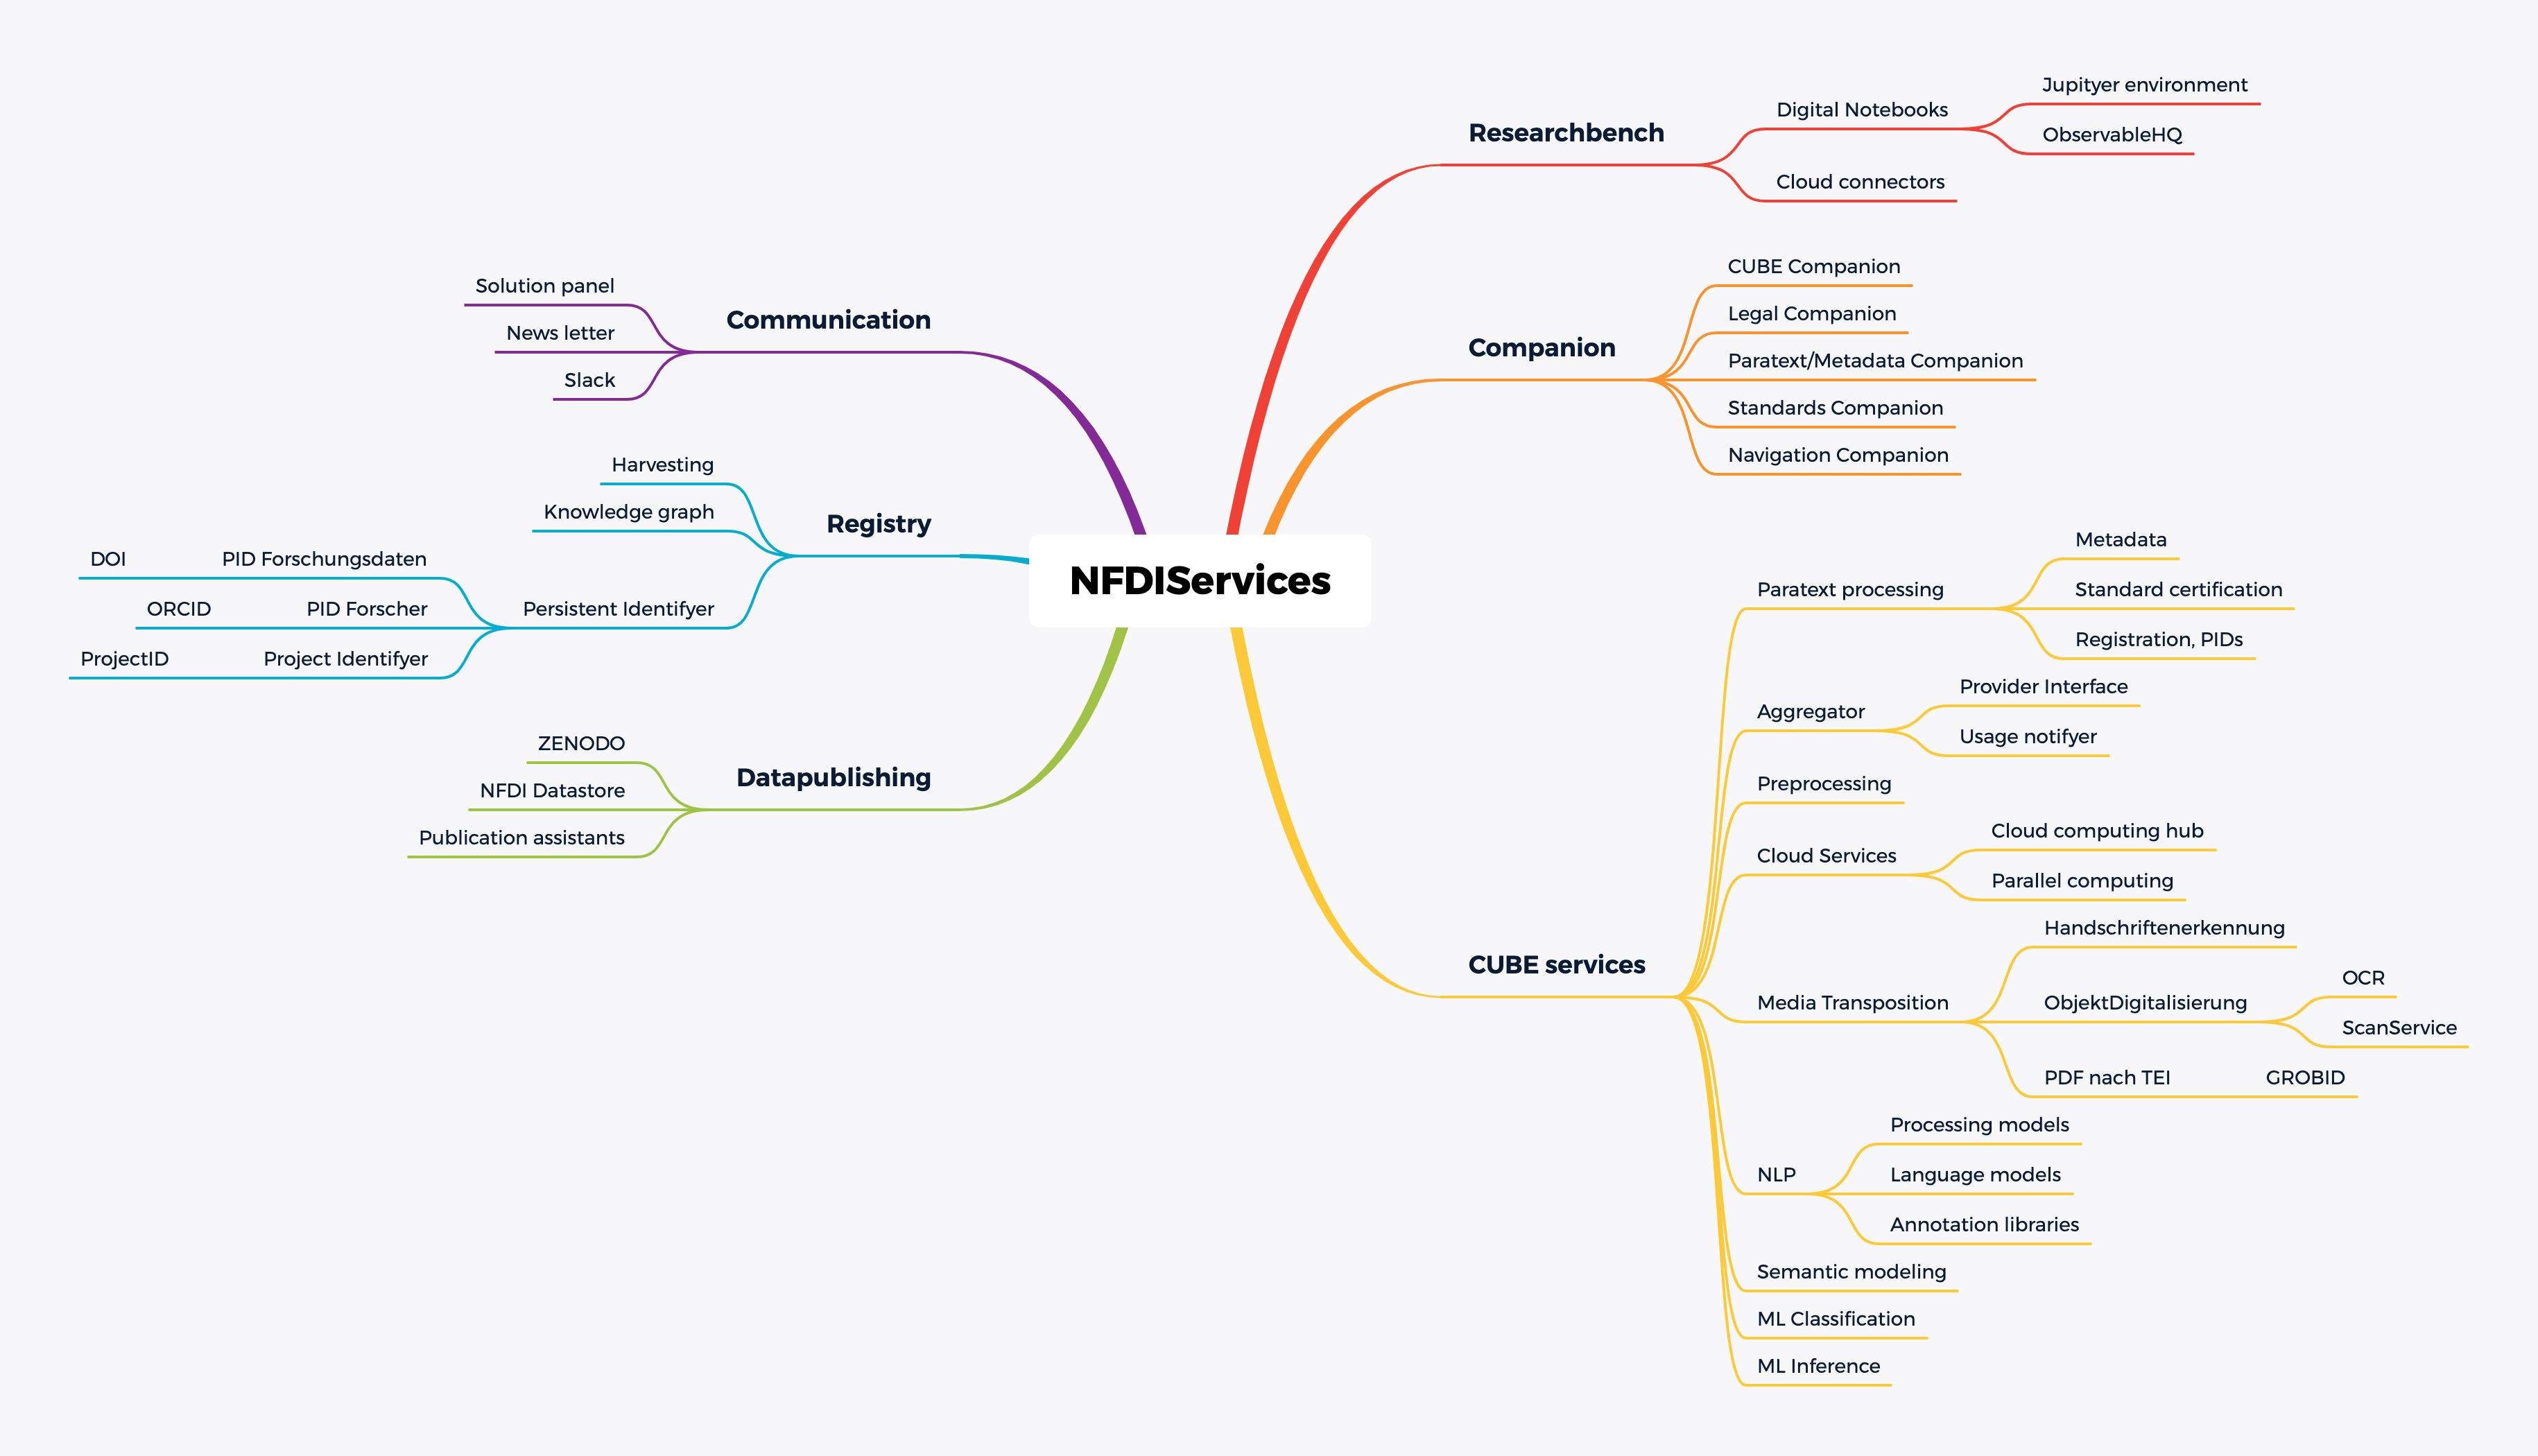
\includegraphics{/Volumes/GGbackup/Dropbox/2020NFDI4SD/Cube/site/services/assets/NFDIServices.png}
\caption{NFDIServices}
\end{figure}

\hypertarget{cube-services}{%
\subsection{Cube services}\label{cube-services}}

\begin{figure}
\centering
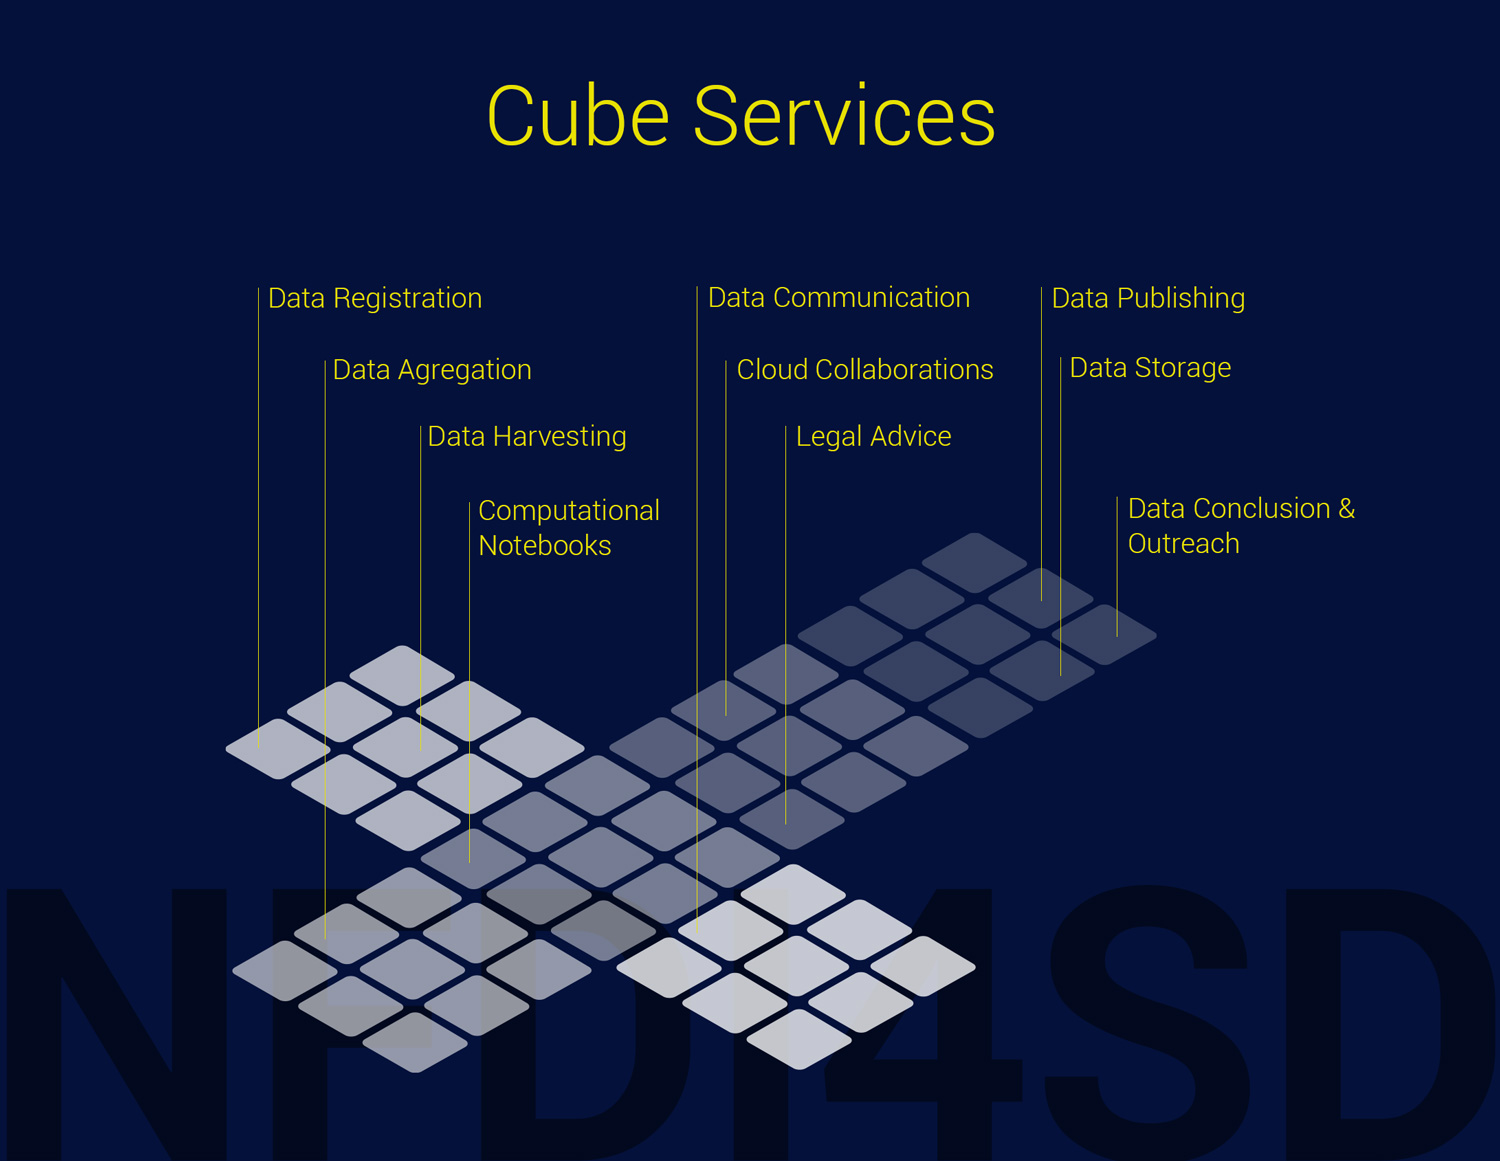
\includegraphics{/Volumes/GGbackup/Dropbox/2020NFDI4SD/Cube/site/services/assets/NFDI4SD_cube-services_1.jpg}
\caption{Cube Servcies}
\end{figure}

NFDI4SD develops a portfolio of cloud services being inspired by goog
practive roles models.

\hypertarget{competing-proposals}{%
\subsection{Competing proposals}\label{competing-proposals}}

\hypertarget{registry-of-research-data-repositories}{%
\subsubsection{Registry of research data
repositories}\label{registry-of-research-data-repositories}}

\begin{itemize}
\tightlist
\item
  \href{https://www.re3data.org}{re3data}
\end{itemize}

\hypertarget{recommended-data-repositories}{%
\subsubsection{Recommended Data
repositories}\label{recommended-data-repositories}}

\begin{verbatim}
- [List of data repositories](https://figshare.com/articles/Scientific_Data_recommended_repositories_June_2015/1434640)
\end{verbatim}

\hypertarget{research-data-publications-of-publishing-houses}{%
\subsubsection{Research data publications of publishing
houses}\label{research-data-publications-of-publishing-houses}}

\begin{itemize}
\tightlist
\item
  \href{https://figshare.com/}{figshare}
\item
  \href{https://www.elsevier.com/authors/author-resources/research-data}{Elsevier}
\item
  \href{https://www.springernature.com/de/authors/research-data}{SpringerNature}
\item
  \href{https://www.springernature.com/de/authors/research-data/research-data-publishing}{SpringerNature
  Data Journals}
\item
  \href{https://www.springernature.com/gp/authors/research-data-policy}{ResearchDataPolicies}
\end{itemize}

\hypertarget{computational-notebooks}{%
\section{Computational Notebooks}\label{computational-notebooks}}

The virtual working environment of NFDI4SD is realised by computational
notebooks. Since 1984, Donald Knuth's paradigm of literate programming
(Knuth \protect\hyperlink{ref-knuth1984a}{1984}) has been based on the
narrative description of algorithms as a weave or mixture of explanatory
text and executable program. Literate programming environments have been
developed for many languages and computational purposes, beginning with
Knuth's own typesetting system.

\hypertarget{jupyter-notebooks}{%
\subsection{Jupyter notebooks}\label{jupyter-notebooks}}

The version of the Jupyter notebooks that is widely used today was
originally developed by Jernando Perez and Brian E. Granger as ``An Open
Source Framework for Interactive, Collaborative and Reproducible
Scientific Computing and Education'' and summarised their objectives in
the points:\footnote{\href{https://ipython.org/_static/sloangrant/sloan-grant.html}{Perez/Granger}}

\begin{quote}
\begin{itemize}
\tightlist
\item
  "Individual exploration: a single investigator tests an idea,
  algorithm or question, likely with a small-scale test data set or
  simulation.
\item
  Collaboration: if the initial exploration appears promising, more
  often than not some kind of collaborative effort ensues.
\item
  Production-scale execution: large data sets and complex simulations
  often require the use of clusters, supercomputers or cloud resources
  in parallel.
\item
  Publication: whether as a paper or an internal report for discussion
  with colleagues, results need to be presented to others in a coherent
  form.
\item
  Education: ultimately, research results become part of the corpus of a
  discipline that is shared with students and colleagues, thus seeding
  the next cycle of research."
\end{itemize}
\end{quote}

Researchers use the NFDI4SD services in the form of advanced
computational notebooks. The researcher can choose from a range of
different running environments of computational notebooks, which are
adapted to the development. NFDI4SD develops comprehensive libraries for
these environments, providing additional functionality for using
research data's computational services, including

\begin{itemize}
\tightlist
\item
  aggregation
\item
  data wrangling
\item
  visualisation
\item
  publication
\end{itemize}

NFDI4SD follows closely the technological development and intends to
support the most important computational notebooks currently used by the
small subjects with the support of the steering committee. The following
figure shows the implementation of computational notebooks by Jupyter
notebooks in the web environment of Jupyterlab.\footnote{\href{https://jupyter.org/}{Jupyter},
  mit \href{https://en.wikipedia.org/wiki/Project_Jupyter}{Wiki} und
  \href{https://jupyterlab.readthedocs.io/en/stable/}{Jupyterlab}.}

Die computational Notebooks entwickeln ihre Funktionalität und
Bedienungsfreundlichkeit ständig weiter.

\begin{itemize}
\tightlist
\item
  Viele verschiedene vielversprechende Ansätze der kollaborativen
  Zusammenarbeit von Forschergruppen an einem Dokument sind bereits in
  fortgeschrittenem Entwicklungsstadium.
\item
  Zukünftige Notebooks kombinieren die Vorzüge aktueller Entwicklungen
  von Computersprachen und gehen flexibel auf die verschiedenen
  Kompetenzfelder der Nutzer ein.
\end{itemize}

Für die Aufgaben der NFDI4SD werden die Anforderungen an open science
research data durch eine erhebliche Erweiterung der Funktionalität von
Notebooks übernommen. Das NFDI4SD entwickelt dazu ein Paket
``Computational Research Objects'' an zusätzlichen Funktionalitäten, in
deren Zentrum die Einführung einer neuen Objektklasse
\emph{CompResearchObject} steht, deren Instanzen alle relevanten
Informationen von Forschungsobjekten alle Attribute beschreibt.

\hypertarget{observablehq}{%
\subsection{ObservableHQ}\label{observablehq}}

Eine sich sehr schnell verbreitende Form von computational Notebooks
sind interaktive Notebooks nach der open source plattform entwickelt von
Mike Bostock - ObservableHQ. Aufbauend auf Bostocks "data driven Für die
Infographics der New York Time perfektionieren diese Notebooks
interaktive Infographiken. ObservableHQ ist ein Repositorium zur
kollaborativen Entwicklung, Austausch und Weiterentwicklung von
visuellen computational Notebooks. Die herausstechenden Graphiken der d3
Bibliothek sind führend im Design und Funktionalität. ObservableHQ
eignen sich ideal zur Visualisierung und Kommunikation von
Forschungsdaten. Aus diesem Grund nutzen führende Medienhäuser diese
Komponenten, neben der New York Times auch Financial Times Graphics, die
in kürzester Zeit mehr als 30 000 Infographiken publizierten. Über die
API der NFDI4SD lassen sich Forschungsdaten direkt in die ObservableHQ
importieren und visualisieren, ohne zwischengeschaltete deployments und
Serverstrukturen.

\href{https://www.ft.com/graphics}{Infographics Financial Times}

\href{https://observablehq.com/@observablehq/user-manual}{Manual}

\hypertarget{collaborative-writing}{%
\subsubsection{collaborative writing}\label{collaborative-writing}}

One can collaboratively write and program computational notebooks in
teams
\href{https://observablehq.com/@observablehq/fork-share-merge?collection=@observablehq/introduction}{Teamwork
with computational notebooks}

\hypertarget{embedding}{%
\subsubsection{embedding}\label{embedding}}

ObservableHQ können schnell und ohne weitere Infrastruktur in andere
Medien eingebettet werden.

\href{https://observablehq.com/@mbostock/embedded-notebook}{Embedding}

\hypertarget{publication}{%
\section{Publication}\label{publication}}

Research data require a publication for their full further use by
others. Thus, the medial spectrum of publication extends to research
data and other media that make direct use of research data. The
methodological requirements for publications such as persistent
identifier, quality assurance, archiving, review, citation, author
attribution or cataloguing remain the same for all publication formats.
Like all forms of publication, data are linked using cross-references to
other publications with full citation and comprehensive bibliographic
references.

\hypertarget{research-data-on-zenodo}{%
\subsection{Research data on Zenodo}\label{research-data-on-zenodo}}

\includegraphics{/Volumes/GGbackup/Dropbox/2020NFDI4SD/Cube/site/services/assets/markdown-img-paste-20200827092932204.png}

NFDI4SD support many data preparation serves to support researchs in
their publication efforts.

\begin{itemize}
\tightlist
\item
  Standardisation: offers transformation into equivalent formats
  reducing variation of terminology and nomenclature.
\item
  Computational assistants check data integrity, completeness,
  consistency
\item
  Publicaton companion as a sophisticated reviewing service to
  interactively prepare research data together with the paratext for
  submission.
\end{itemize}

We encourage the use of a newly created \emph{NFDI4SD Community
Collections} for text and data publications. As an example: the SAO/NASA
Astrophysics Data System supports the publication of astronomy thesis in
\href{https://zenodo.org/communities/astrothesis?page=1\&size=20}{Zenodo's
Astronomy Thesis Collection}.

At the same time Zenodo both allows bulk uploading and harvesting its
repositories. The policy allows NFDI4SD to implement a rapid open
science publication workflow for its research bench implementation. A
curated publishing setup from the implementation of NFDI4SD provides the
best of two worlds for researchers using NFDI4SD services: research data
will be curated and scrutinized by NFDI4SD research data compliances.
Machine learning diagnostic tools support the composition of research
data before they will be submitted for publication. Enhanced research
metrics will supplement the NFDI4SD registry to document, display and
facilitate collaborative usage of published research data by others.

Creation of a DOI registered data submission on Zenodo ist
straightforward and well established.\footnote{\href{https://guides.github.com/activities/citable-code/}{submitting
  to ZENODO}}

\includegraphics{/Volumes/GGbackup/Dropbox/2020NFDI4SD/Cube/site/services/assets/markdown-img-paste-20200831120756335.png}

\hypertarget{research-data-publication-of-repositories}{%
\subsection{Research data publication of
repositories}\label{research-data-publication-of-repositories}}

NFDI4SD will be instrumental in setting up large digital repositories.
Depending on the size of data and demand of overall storage capacity
designed recommendations and interfaces for long term data repositories
will be provided. During the pilot period all existing large data
repositories will be evaluated for its suitability and a matrix of
evaluation criteria will be published.

\hypertarget{interactive-articles}{%
\subsection{Interactive articles}\label{interactive-articles}}

Development of interactive articles is rapid with many scholarly
attributes like mathematical typsetting, tables, crossreferences,
footnotes and bibliographies including extended bibliographies of
published research data. NFDI4SD will adopt and develop one interactive
article framework with simlar objective as
\href{https://distill.pub/journal/}{distill journal} with
\href{https://distill.pub/guide/}{distill guide}. A brilliant article
about advantages of interactive articles has been published by
\href{https://distill.pub/2020/communicating-with-interactive-articles/}{Hohmann,
Conlen, Heer and Chau.}

However, destill's authoring process has to be much simplified and
especially expandedfor integrating research data publication. We believe
that interative articles are the perfect platform for documenting and
explaining published datasets.

\includegraphics{/Volumes/GGbackup/Dropbox/2020NFDI4SD/Cube/site/services/assets/markdown-img-paste-2020091408134547.png}

NFDI4SD will develop an much more accessible authoring system with
zero-additional-skill manuscript writing and support for extending
research data inclusion. It will transform the presentation of research
data beyond traditional forms of documentation.

\hypertarget{content-partner}{%
\section{Content Partner}\label{content-partner}}

\hypertarget{content-provider}{%
\subsection{Content provider}\label{content-provider}}

Researchers use a dense network of research data. The small subjects are
dependent on research data from a wide range of disciplinary sources.
NFDI4SD provides software packages for computational notebooks that can
import, cite and reuse the diverse data offered by providers. The
employed research data are used in data links, algorithmic derivation or
combined data sets. Linked data is an essential part of the research
work. In their combination, the NFDI4SD provides invaluable support for
automated access to required research data.

\begin{itemize}
\tightlist
\item
  Data aggregation: Research objects of one species are often required
  on a large scale, often as representative sample data: Documents on a
  topic are rarely found already prepared and compiled in one data
  source. Even very large libraries and archives seldom maintain
  complete collections. Most research projects depend on their own
  consolidation of the research subjects and preparation of the data in
  suitable data formats.
\end{itemize}

\hypertarget{table-of-envisaged-provider}{%
\subsection{Table of envisaged
provider}\label{table-of-envisaged-provider}}

\hypertarget{research-organisation}{%
\chapter{Research Organisation}\label{research-organisation}}

\hypertarget{objectives-and-task-areas}{%
\section{Objectives and Task Areas}\label{objectives-and-task-areas}}

\hypertarget{section}{%
\section{}\label{section}}

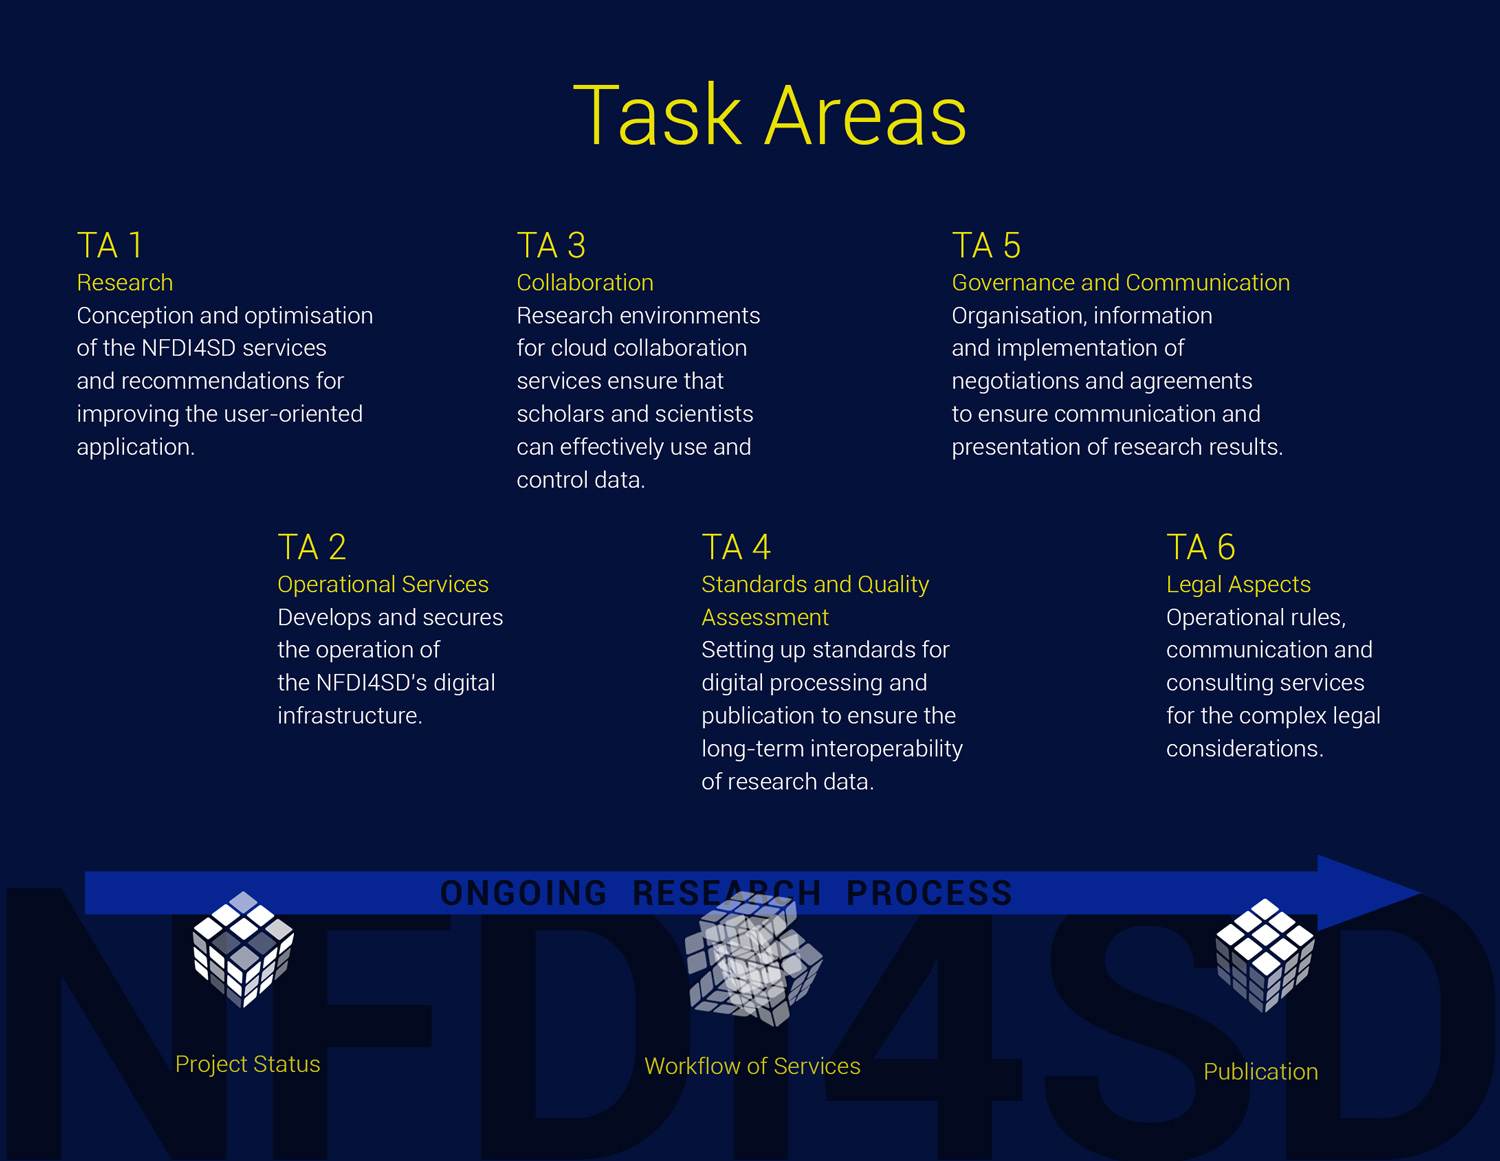
\includegraphics{/Volumes/GGbackup/Dropbox/2020NFDI4SD/Cube/site/research/assets/NFDI4SD_task-areas.jpg}

Digital transformation is fundamentally changing the way researchers
work, particularly in the small disciplines. These scholars are
typically involved in highly collaborative and global long-term projects
that use innovative technology, but they often do not have access to the
research data and publication infrastructure that their home
institutions usually provide to researchers. Collaborative projects
require agile workflows for all user groups. Data aggregation,
preparation, processing, analyses and publications are all important
elements of modern scholarly research. The main purpose of the NFDI4SD
consortium is to provide scholars with research-integrating data
together with other scientific support. By concentrating on the small
disciplines, the consortium will be able to supply researchers with the
services they require on a daily basis. The first objective will be to
break up the traditional, sequential way in which the research procedure
is organised and weave the research data, including publication of the
data, into an integrated research process, complemented by a moderated
research model that incorporates research data into the ongoing research
workflow (or, as we call it, the `cube').

\hypertarget{objectives}{%
\subsection{Objectives}\label{objectives}}

\begin{awesomeblock}[magenta]{1pt}{O1}{magenta} Both the use and production of research data will be tightly integrated into ongoing research projects. Since antiquity, science research has been an collaborative enterprise. The NFDI4SD’s services will become an integral part of current research, initially through the NFDI4SD entering into collaboration with new research projects. These agreements will be open to all disciplines, independent of their institutional classification as ‘small disciplines’.\end{awesomeblock}

Currently, the main desideratum of researchers working in the small
disciplines is access to modern computational research data beyond the
support of their home institutions and third-party funding bodies. As
science is per se a collaborative undertaking, knowledge exchange is
fundamental to developing innovative and critical science. As a support
infrastructure, the NFDI4SD will be a novel institutional research
partner in the scientific arena.

\begin{awesomeblock}[magenta]{1pt}{O2}{magenta} The NFDI4SD will develop research data services that respond directly to the feedback of research projects. For many years now, the Arbeitsstelle Kleine Fächer (Small Disciplines’ Unit) has been recording the institutional framework of the small disciplines. It enables researchers, students, institutions and, in the future, the NFDI4SD to communicate directly with one another. New concepts in the computational philosophy of science will guide the software architecture of research data flows.\end{awesomeblock}

Computational tools develop at a rapid pace. NFDI4D aims to use the
latest of those and motivate its researcher to deploy their own for
common use as quickly as possible.

\begin{awesomeblock}[magenta]{1pt}{O3}{magenta} The NFDI4SD will use and develop best-practice, open-source tools and computational libraries to provide their services within the European Open Science Cloud (EOSC).\end{awesomeblock}

The NFDI4SD will be an active member of the German NFDI consortium and
will strive to form collaborations with other suitable consortia. It
will commit itself to the strategic plans of the EOSC Roadmap and seek
membership in the newly created EOSC Association. The proven
infrastructure of CERN's Zenodo platform will provide OpenAIRE data
publication, data harvesting and it will adhere the FAIR data principles
in order to realise the eight ambitions of Open Science.

\begin{awesomeblock}[magenta]{1pt}{O4}{magenta} The signing of agreements with relevant stakeholders – libraries, archives and other content providers – on standards, application programming interfaces (APIs) and open access via computer networks.\end{awesomeblock}

The NFDI4SD governing body will seek to enter into operational
agreements with a several content-providing institutions on the
implementation and accessibility of APIs for the NFDI4SD's
infrastructure hub. These agreements, using widely accepted standards,
will enable researchers to access large sets of research data from a
large number of content-holding institutions. It is expected that,
within a short space of time, the NFDI4SD will be able to provide
standardised API and interface modules. The large variety of small
disciplines involved will ensure that special collections beyond the
significant stakeholders will be included in this integrated network of
content providers.

\begin{awesomeblock}[magenta]{1pt}{O5}{magenta} The NFDI4SD aims to maximise the visibility of the impact of research\end{awesomeblock}

New generation metrics monitors will be implemented to monitor the use
and impact of the NFDI4SD's services as part of the support offered to
research projects. Daily, updated monitors and impact indicators will
enable researchers to assess their collaborative global network as well
as to inform the NFDI4SD's governing body of hotspots of usage and of
the need to steer users towards a particular course of action.

\begin{awesomeblock}[magenta]{1pt}{O6}{magenta} Publication and science outreach\end{awesomeblock}

All output for general scholarly use will be regarded as publishable
material. Such material goes beyond putting data on a file server:
publications adhere to FAIR data principles and use review, curation and
scholarly assessments. The NFDI4SD intends to establish new procedures
and references for data publications so as to significantly enhance the
impact of research.

\hypertarget{task-areas}{%
\subsection{Task areas}\label{task-areas}}

The nature, benefits and characteristics of research data are
surprisingly complex: data exist in many different media formats and
contribute to the information value of the subject areas of research,
while researchers benefit from the speedy dissemination of their
publications and research findings, which leads to rapid knowledge
exchange. A Research Management Plan will coordinate the use and
interoperability of the NFDI4SD's services. Internal and external forms
of communicating for research purposes, data storage, usage and revision
as well as full-page archiving, including the publication of the
research findings and research data, will all form part of the NFDI4SD's
services.

The workflow of research activities in the context of highly
collaborative, agile scientific communities occurs at the interplay
between data and theory, using -- among other things -- computational
means. Such activities can neither be ordered as a linear sequence of
tasks, nor as a research data life cycle. The organisation of the
workflow of research activities has been designed using Thomas Kuhn's
metaphor of science as a puzzle-solving activity. We describe the
pipeline of scientific processes as the transformation of input data via
research pipes into designed outcomes. This operational sequence can be
compared to the rotations of a multidimensional research cube (solving
Rubik's cube, for example). The cube's faces represent the content,
data, skills, or means of the research activities. Each single step
(that is, each rotation of the cube) leads to a new configuration.

This puzzle-solving metaphor facilitates the orchestration of the
NFDI4SD's services into research activities by organising and
communicating the growing repertoire of the NFDI4SD's numerous research
data services. The cube describes the requirements, standards and
quality of data as well as the information, metadata and documentation
they contain, in order to assure the best usage of services. The NFDI4SD
is basing its operation on a wide spectrum of standards, API norms, data
formats as recommended by the EOSC and other standard institutions. The
NFDI4SD will rapidly develop a user-friendly service catalogue that will
serve as a graphical user interface (GUI) for researchers, who will be
able to choose their needed service, quickly apply it to their given
data and research questions and then obtain their findings.

\begin{awesomeblock}[magenta]{1pt}{TA1}{magenta} research\end{awesomeblock}

The aim of this large task area is to observe at close range the
application of the NFDI4SD's services and then to recommend the
development of additional services to satisfy the demands of the various
disciplines. TA1 will be supported by a broad range of fields, assisted
by coordinators.

\begin{awesomeblock}[magenta]{1pt}{TA2}{magenta} operational services\end{awesomeblock}

This operational task area is to develop and secure the running of the
NFDI4SD's infrastructure, using Zenodo, Europe's renowned research data
publishing platform.

\begin{awesomeblock}[magenta]{1pt}{TA3}{magenta} collaboration\end{awesomeblock}

There is a rising demand for cloud collaboration services among today's
research environments. The direct exchange of information is being
replaced by the publication of texts and data, with user interfaces
ensuring that scholars and scientists can use and control data
effectively, without having to undergo any special training. In
addition, metadata as well as knowledge graphs, advanced catalogues and
reference tools will enable users of the NFDI4SD's services to make the
most of open scientific data.

\begin{awesomeblock}[magenta]{1pt}{TA4}{magenta} standards and quality assessment\end{awesomeblock}

Data encoding, flow computers, computer interfaces, APIs and
publications require widely applicable standards, norms and metadata.
Our principal investigators (PIs) are long-term members of the key
standardisation committees and so will ensure the interoperability of
the research data over a long period of time.

\begin{awesomeblock}[magenta]{1pt}{TA5}{magenta} governance and communication\end{awesomeblock}

The highly experienced and international scientific representatives
responsible for this TA will ensure that there is an effective
information flow and that negotiations and agreements with research
institutions around the world proceed smoothly. Virtual conferences,
newsletters, blogs and, hopefully, physical meetings in the
not-to-distant future should promote productive and effective science
communication, including the transmission of science findings to the
general public.

\begin{awesomeblock}[magenta]{1pt}{TA6}{magenta} legal aspects\end{awesomeblock}

Intense scientific collaborative work and the exchange of information,
including the publication of data, involve complex legal considerations.
This area will be tasked with preparing the operating rules, virtual
information desks and consultation services. It will also actively shape
the future legal landscape of the research process in the digital age.

\hypertarget{measures-and-workpackages}{%
\section{Measures and Workpackages}\label{measures-and-workpackages}}

\hypertarget{work-program}{%
\section{Work program}\label{work-program}}

\hypertarget{terminology}{%
\subsection{Terminology}\label{terminology}}

DFG proposed using the following terminology, services and work
programme:

\begin{quote}
\textbf{Services:} In describing the services to be provided by the
consortium, distinguish clearly between services that consortium members
will provide as part of their institutional mission (Grundaufgaben)
based on existing funding, and new services that will be established
within the NFDI framework (and for which funding can be requested within
the NFDI).
\end{quote}

\begin{quote}
\textbf{Work Program:} This section describes the structure of your work
programme as it relates to the specific \textbf{aims} and
\textbf{objectives} of the proposed consortium, particularly to your
research data management strategy. Major achievements to be attained
during the course of the work programme, such as community-wide
standards, can be defined as \textbf{milestones.} Tangible results, such
as defined services, can be categorised as \textbf{deliverables.}
\end{quote}

\begin{quote}
The work programme of a consortium is divided into \textbf{task areas},
which may consist of different \textbf{measures.} Please provide
\textbf{tabular overviews} of the envisaged task areas, the proposed
\textbf{measures per task area}, and the \textbf{individual(s)
responsible for a given task area (co- spokespersons)}. Provide a
detailed description of the measures to be addressed in the task area
and explain how they relate to your specific objectives. Explain the
contribution of the consortium members and/or participants who will be
involved in the individual measures.
\end{quote}

\begin{quote}
\textbf{Mark task areas that are relevant to other NFDI consortia} or
will be applied for within other consortia accordingly and explain the
relation (e.g.~by using footnotes or text below the table).
\end{quote}

\begin{quote}
The coordination and \textbf{administrative tasks for the consortium as
a whole} must be included in a separate task area --usually the
concluding one. Note that applicants may request funds to coordinate
activities or work with other consortia. ``Provide a detailed
description of the measures to be addressed in the task area and explain
how they relate to your specific objectives. It may be helpful to work
with or develop use cases to illustrate your approach. Which aspects of
your research data management strategy will be addressed by this task
area? Explain the contribution of the consortium members and/or
participants who will be involved in the individual measures. How will
this task area cooperate with other task areas (include cross-area
dependencies where applicable)? Address possible risks of
implementation.''
\end{quote}

Task Areas

Measures

Tasks

Responsibilities

TA 1 Research

M1.1 -- Working Group: Wunschkonzerte ``Wunschkonzerte'' ist eine
Veranstaltungsreihe mit Kurzpräsentationen der Nutzer zur erhofften
Weiternutzung ihrer Forschungsdaten durch andere und dem gewünschten
Beitrag des NFDI4SD. Das jährliche „Prom`` stellt ausgewählte
Wunschkonzerte und die Neuerung des NFDI4SD vor.

T1.1.1: Organisation Konzert

Jürgen Renn, Dagmar Schäfer, Carolin OdebrechtKärin Nickelsen

T1.1.2: Konzert Publikation + Kommunikation

T1.1.3: Promenadenkonzert, Evaluation, Bericht Umsetzung

M1.2 -- Working Group: Projektauswertung

T1.2.1:Kommunikation NFDI4SD mit Projekten über Nutzenund Bedarf

T1.2.2: Definition der Desiderate an NFDI4SD Services

T1.2.3: Evaluation der Nutzungsmetriken bezogen auf Nutzer

M1.3 -- Working Group: Neue Nutzerkreise

T1.3.1: Auswertung laufende Forschungsprojektenational/international

T1.3.1: Identifikation ungenutzte Datenprovider

T1.3.3: Regelmäßig erscheinende Newsletter für offene Abonnentenkreise

TA 2 Operational Services

M2.1 -- Working Group: Develops and secures the operation of the
NFDI4SD'sinfrastructure (Big Data, Machine Learning and so forth).

T2.1.1:

Klaus-Robert Müller, Jürgen Renn,Gerd Graßhoff(Support CMS HU Berlin)

T2.1.2:

T2.1.3:

M2.2. -- Working: Data publishing

T2.2.1:

T2.2.2:

M2.3 -- Working: Data harvesting and storage

T2.3.1:

T2.3.2:

TA 3 Collaboration

M3.1 -- Working Group: Research environments for cloud collaboration
services ensure that scholars and scientists can effectively use and
control data (including metadata, knowledge graphs, advanced catalogues,
and reference tools).

T3.1.1:

Markus Hilgert,Christof Schütte

T3.1.2:

T3.1.3:

M3.2 -- Working Group:

M3.3 -- Working Group:

TA 4 Standards and Quality Assessment

M4.1 -- Working Group: Setting up standards for digital processing and
publication to ensure the long-terminteroperability of research data.

T4.1.1:

Uwe SchmidtGerd Graßhoff

T4.1.2:

T4.1.3:

M4.2 -- Working Group:

M4.3 -- Working Group:

TA 5 Governance and Communication

M5.1 -- Working Group: Organization, information andimplementation of
negotiations and agreements toensure communication and presentation of
research results.

T5.1.1:

Andreas Degkwitz, Klaus Ceynowa,

T5.1.2:

T5.1.3:

M5.2 -- Working Group:

T5.2.1:

M5.3 -- Working Group:

T5.3.1:

TA 6 Legal Aspects

M6.1 -- Working Group: Rechtsdiagnostik betroffenerBereiche
Forschungsdaten

T6.1.1: Urheberrecht

Eva Inés Obergfell

T6.1.2: Persönlichkeitsschutzrechte

T6.1.3: Datenschutz-Grundverordnung der EU (DSGVO)

M6.2 -- Working Group: Dokumentation, Hilfestellungen

T6.2.1: Zusammenstellung Sammlung Dokumente, Informationsmaterial

T6.2.2: Newsletter mit Info-Telegramm

M6.3 -- Working Group: Automatisierte Analyse/Companion

T6.3.1: Regelentwicklung

T6.3.2: Companion Rechts-Analyse Forschungsdaten

T6.3.3: Evaluation Performanz Companion

\hypertarget{user}{%
\section{User}\label{user}}

NFDI4SD zielt darauf ab, von der großen Nutzergruppe der Forscher der
Kleinen Fächer wie auch andere Interessierte auf ihre Bedürfnisse an
Leistungen der Forschungsdateninfrastruktur hingewiesen zu werden. Mit
Beginn der Arbeiten wird das NFDI4SD

\hypertarget{forscher-laufend-informieren}{%
\subsection{Forscher laufend
informieren}\label{forscher-laufend-informieren}}

\begin{itemize}
\item
  alle Forscher und Projektmitglieder kontaktieren
\item
  über die Serviceangebot informieren
\item
  in Medien, Blogs und sozialen Medien über die Angebote orientieren
\item
  abonnierte News Dienste einrichten
\end{itemize}

\hypertarget{uxfcber-forschungsdaten-informieren}{%
\subsection{Über Forschungsdaten
informieren}\label{uxfcber-forschungsdaten-informieren}}

Die Forschungsdaten werden maximal sichtbar katalogisiert und seine
Metadaten in die relevanten Dienste integrieren. Größere Repositorien,
institutionelle Repositorien oder historisch gewachsene Datenbestände
werden von eigenen IT-Einrichtungen betrieben und über API in die
Forschungsdatenschnittstellen des NFDI4SD eingebunden. Dazu werden mit
den Institutionen geeignete Abkommen abgeschlossen.

\hypertarget{nfdi4sd-general-repository}{%
\subsection{NFDI4SD general
repository}\label{nfdi4sd-general-repository}}

Das NFDI4SD verwendet community Ressourcen und schlägt die Nutzung von
ZENODO als Publikationsplattform für Communities als eine der
präferierten Plattformen als general repository für kleinen bis mittlere
Datenbestände vor. Diese werden insbesondere für die sekundären
Forschungsdaten besonders relevant.

\hypertarget{comparison-of-general-research-data-repositories}{%
\subsection{Comparison of general research data
repositories}\label{comparison-of-general-research-data-repositories}}

\begin{quote}
The General Repository Comparison Chart and FAIRsharing Collection
(https://fairsharing.org/collection/GeneralRepositoryComparison) is an
outcome of the NIH Workshop on the Role of Generalist Repositories to
Enhance Data Discoverability and Reuse held 11-12 February 2020
(workshop summary). Following the workshop, representatives of the
participating generalist repositories collaborated to develop a tool
researchers could use to make decisions about selecting a general
repository. We intend for the content to be dynamically updated through
our partnership with FAIRsharing. As we work towards that goal, we
currently have a static version of the comparison.\footnote{\href{https://www.rd-alliance.org/groups/generalist-repository-comparison-chart-management-group}{RDA
  management group}}
\end{quote}

\hypertarget{impact-of-zenodo}{%
\subsection{Impact of Zenodo}\label{impact-of-zenodo}}

Studie zum Impact für Forschungsdaten Stall et al.
(\protect\hyperlink{ref-stall2020a}{2020})

\hypertarget{discovery-for-software-and-data}{%
\subsection{Discovery for software and
data}\label{discovery-for-software-and-data}}

Nutzungsweise bestehender Forschungdateninfrastruktur zur Suche Nielsen
et al. (\protect\hyperlink{ref-nielsen2018}{2018}):

\hypertarget{communities-on-zenodo}{%
\subsection{Communities on zenodo}\label{communities-on-zenodo}}

-https://zenodo.org/communities/o2r/?page=1\&size=20 +
https://gepris.dfg.de/gepris/projekt/142173438/ergebnisse +
https://gepris.dfg.de/gepris/projekt/96214342/ergebnisse

\hypertarget{epistemology}{%
\section{Epistemology}\label{epistemology}}

\hypertarget{epistemology-of-research-data-1}{%
\section{Epistemology of research
data}\label{epistemology-of-research-data-1}}

\hypertarget{observablehq-20a6021f}{}

The epistemological network of the NFDI4SD will be a novelty. Research
data are usually published in logical isolation and, if necessary,
searched through cataloguing categories. In the visualisation, different
objects of research data are classified by category in a thematic cube.
The registry of the NFDI4SD enhances browsing in research data
catalogues. It uses machine learning methods to create relationships
between the data: Provenance or inferential relationships. These
networks are created for all catalogued research data, not only those
for which researchers have used the services of the NFDI.Similar to
citation graphs of citations between publications, all accessible
publications of research data are referentially linked with machine
learning tools.

Deep learning models reveal the content and classify the research data
on which the argumentation of the publications is epistemically
based.These searches are initially prepared for the small subjects and
can offer very substantial and specific support for the research
projects. The registry of the NFDI4SD creates a special
\textbf{epistemic knowledge graph} for the most diverse contexts of
research data:

\hypertarget{impact-analysen}{%
\subsection{Impact Analysen}\label{impact-analysen}}

Usage relationships between research data show the wide range of uses.
In the following diagram, the usage strands are represented by different
widths of the zones.

\hypertarget{observablehq-89935fa8}{}

\hypertarget{governance}{%
\chapter{Governance}\label{governance}}

\hypertarget{bodies}{%
\section{bodies}\label{bodies}}

\hypertarget{consortium}{%
\section{Consortium}\label{consortium}}

\begin{figure}
\centering
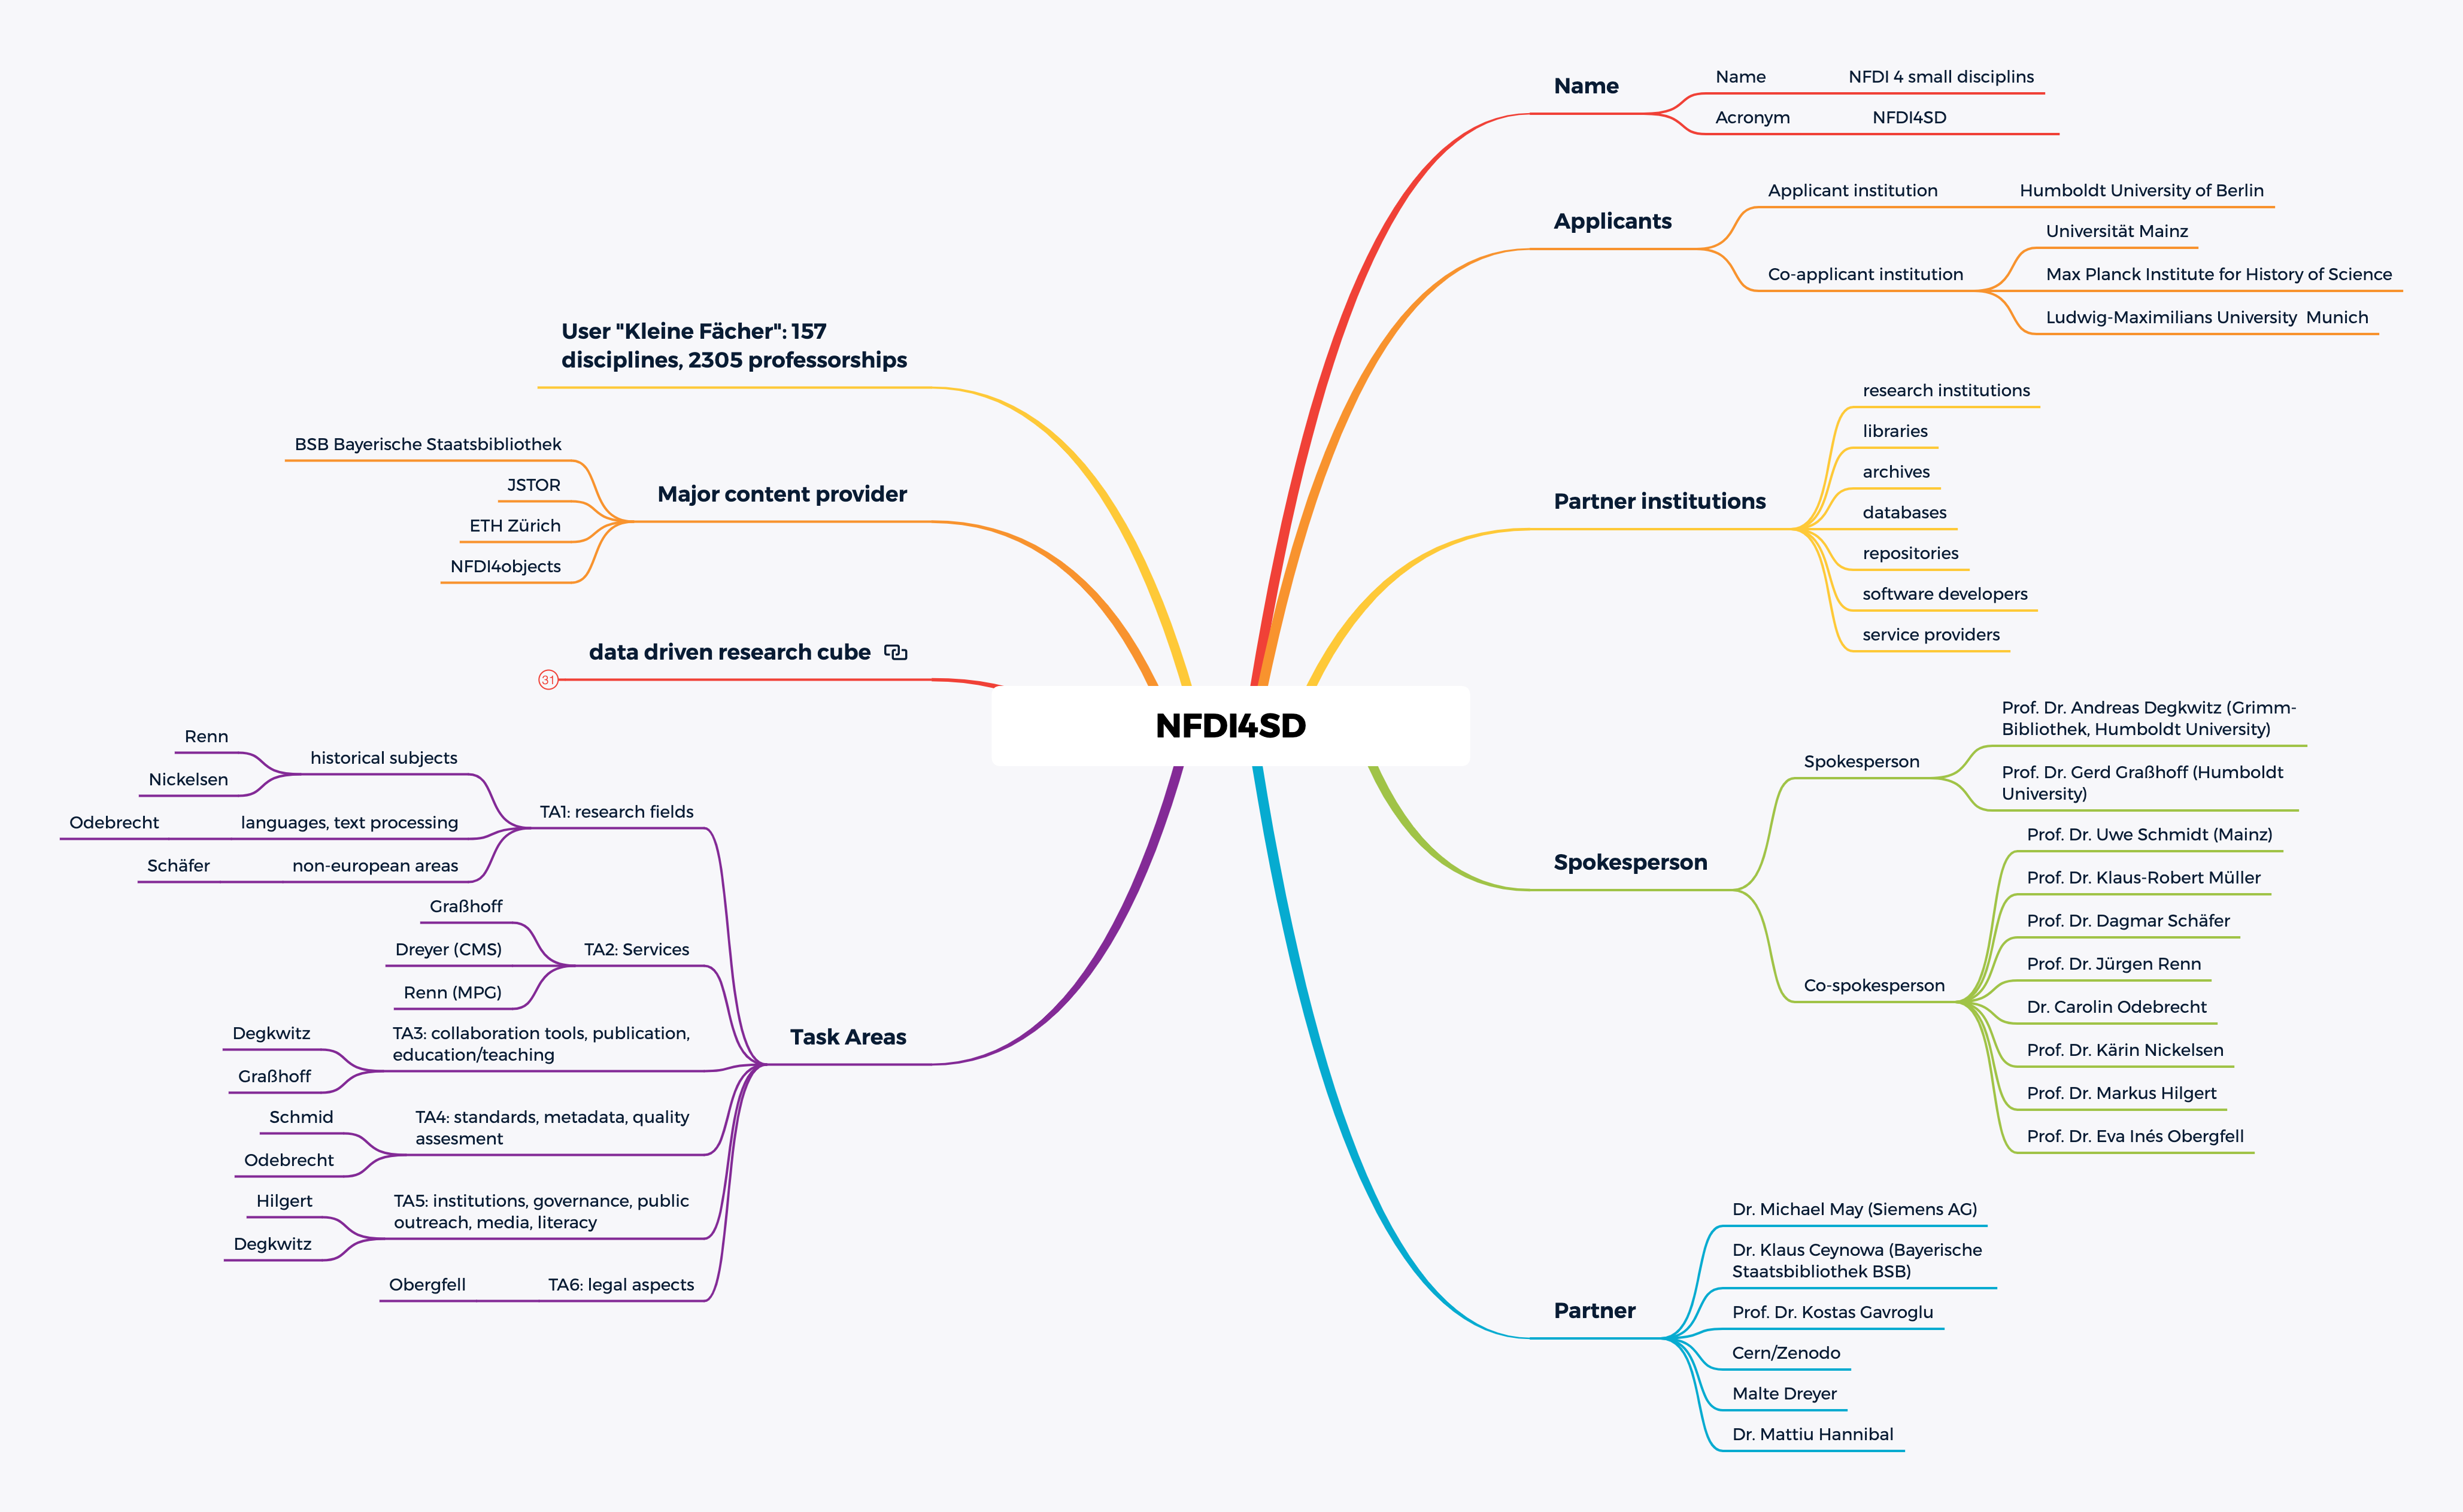
\includegraphics{/Volumes/GGbackup/Dropbox/2020NFDI4SD/Cube/site/governance/assets/NFDI4SD.png}
\caption{NFDI4SD}
\end{figure}

All spokespeople are members of the \textbf{steering committee} which
regularly reviews and decides per majority - timeline of workpackages -
major working contracts - user feedback and requests - evaluation of
performance metrics - new members, partners, advisors, workshops and
conferences - spokespeople responsible for TAs and working packages
report to the steering committee and place their proposal for
consideration - decide about annual budget - The two spokespeople are
responsible for the daily administrative decisions on issues which are
defined by the \textbf{steering committee} at the inauguration of the
NFDI4SD.

\textbf{task areas} have responsible spokespeople confirmed and assigned
by the steering committee. Their goals and milestones are defined in the
\textbf{table of tasks} submitted with the NFDI4SD proposal. Its
composition will be reviewed and decided on by the \textbf{steering
committee} annually, if needed on shorter notice.

A \textbf{scientific advisory board} will be elected with the
inauguration of the NFDI4SD by the \textbf{steering committee}. It will
advice the steering committee on requests and report to the body
regularly.

The applicant institution is legaly responsible to the DFG. Budgets for
staff employed by co-applicant institutions are transfered according to
DFG procedures.

\textbf{Partner institutions} and \textbf{content provider} may signed
contracts or letter of understanding for services for NFDI4SD such as
access regulations and usage permits. These contracts are prepared by
TA5 and administered by the applicatant instituion.

A \textbf{pilot period} from January 2021 until a project inauguration
time will conduct workshops, review potential staff and organize
meetings of the steering committee to consider recommendations for the
inauguration meeting. External experts and advisors can be consulted for
reviewing the working plan up to the inauguration of the NFDI4SD.
Additional funding might support preparatory studies and developments.

\hypertarget{forms-and-regulations}{%
\section{Forms and regulations:}\label{forms-and-regulations}}

\begin{itemize}
\tightlist
\item
  \href{https://www.dfg.de/foerderung/programme/nfdi/formulare_merkblaetter/index.jsp}{DFG
  NFDI Merkblätter}
\item
  \href{https://www.dfg.de/formulare/nfdi120/nfdi120_en.pdf}{Funding
  criteria}
\item
  \href{https://www.dfg.de/formulare/nfdi130/nfdi130_en.pdf}{Compliance
  form}
\item
  \href{https://www.dfg.de/formulare/nfdi300/nfdi300_de.pdf}{Verwendungsrichtlinien}
\item
  \href{https://www.dfg.de/download/pdf/foerderung/antragstellung/elan/flyer_eant_de.pdf}{Elan
  flyer}
\end{itemize}

\hypertarget{budget-summary}{%
\section{Budget summary}\label{budget-summary}}

Staff will be appointed by the applicant institutions in line with the
\href{https://www.dfg.de/formulare/60_12/60_12_de.pdf}{Personalmittelsätze
DFG}. Institutions will supply the required working facilities. The main
applicant institution will provide adminstrative facilities for the
NFDI4SD. Co-applications will have no additional financial and
structural obligation beyond these commitments as described in the
submitted detailed budget plan.

\hypertarget{bibliography}{%
\section{bibliography}\label{bibliography}}

\hypertarget{bibliography-1}{%
\section*{Bibliography}\label{bibliography-1}}
\addcontentsline{toc}{section}{Bibliography}

\hypertarget{refs}{}
\begin{cslreferences}
\leavevmode\hypertarget{ref-zotero-40395}{}%
``Annika Rockenberger, PhiN 76/2016: 20.'' n.d.
http://web.fu-berlin.de/phin/phin76/p76t2.htm\#fz16.

\leavevmode\hypertarget{ref-genette1997}{}%
Genette, Gerard. 1997. \emph{Paratexts: Thresholds of Interpretation}.
Cambridge University Press.

\leavevmode\hypertarget{ref-knuth1984a}{}%
Knuth, D. E. 1984. ``Literate Programming.'' \emph{The Computer Journal}
27 (2): 97--111. \url{https://doi.org/10.1093/comjnl/27.2.97}.

\leavevmode\hypertarget{ref-nielsen2018}{}%
Nielsen, Lars Holm, August Muench, Alberto Accomazzi, Krzysztof Nowak,
Alexandros Ioannidis, Sergi Blanco-Cuaresma, Edwin A. Henneken, Jose
Benito Gonzalez Lopez, and Julie Steffen. 2018. ``Asclepias: Enabling
Software Citation and Discovery.''
\url{https://doi.org/10.5281/zenodo.1283381}.

\leavevmode\hypertarget{ref-stall2020a}{}%
Stall, Shelley, Maryann E. Martone, Ishwar Chandramouliswaran, Mercè
Crosas, Lisa Federer, Julian Gautier, Mark Hahnel, et al. 2020.
``Generalist Repository Comparison Chart,'' July.
\url{https://doi.org/10.5281/zenodo.3946720}.

\leavevmode\hypertarget{ref-unold2019}{}%
Unold, Martin, Florian Thiery, and Allard Mees. 2019. ``Academic Meta
Tool Ein Web-Tool zur Modellierung von Vagheit.'' In \emph{Die
Modellierung des Zweifels Schlüsselideen und -konzepte zur
graphbasierten Modellierung von Unsicherheiten.}, edited by Andreas
Kuzera and Thorsten Wübbena. Zeitschrift für digitale
Geisteswissenschaften. Wolfenbüttel.
\end{cslreferences}

\backmatter
\end{document}
